
%--------------- Chapter 4: DiversityAnalysis ---------------%

\chapter{OPTIMAL CODEBOOK CONSTRUCTION}\label{Ch4:codebookconstruction}
\graphicspath{{Chapter4/Chapter4Figs/}{Chapter4/Chapter4Figs/}}

\section{Introduction}\label{ch4:sec:Intro}


The effectiveness of the BOF method is highly dependent on the formed visual vocabulary which is generated by the clustering of feature descriptors in the codebook construction phase. Clustering, an optimization problem, is a method to assign all the data points to certain clusters by using minimum cohesion or maximum separation. For the same, K-means clustering is generally employed to cluster feature vectors as it is computationally fast. However, it may generate biased centers when applied to high dimensional descriptor space extracted from tissue images. Therefore, there is a requirement of generating optimal visual words that are not biased and this can be achieved with the use of optimization algorithms that can work well for the clustering problem.  In literature, various meta-heuristic methods have exhibited better performance for clustering  \cite{bong2012} \cite{ahmed2017}. Out of these, biogeography-based optimization (BBO) \cite{Simon2008} is one of the popular methods based on island biogeography and is used effectively in clustering problems and computer vision applications \cite{ma2017}. However, BBO also suffers from some demerits like single feature migration property, poor population diversity, and sticking into local optima sometimes \cite{lim2016}. To mitigate these demerits, two new variants of BBO, namely improved biogeography-based optimization (IBBO) and spiral biogeography-based optimization (SBBO) are introduced in this chapter which is described in the following sections. Further, these variants are used to generate the optimal visual vocabulary in the BOF method which is used to classify the histopathological images. The modified BOF method with the optimal codebook construction method is shown in Figure \ref{ch4:fig:codebook}.

\begin{figure}[h!]
            \centering
            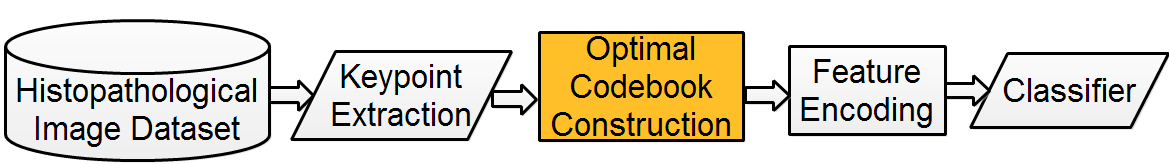
\includegraphics[width=0.8\textwidth]{codebook}
            \caption[Flow chart of the BOF method with modified codebook construction]{\fontsize{10}{12} \selectfont Flow chart of the enhanced BOF method with optimal codebook construction}\label{ch4:fig:codebook}
\end{figure}

\section{Biogeography-based Optimization Algorithm} \label{ch4:sec:bbo}

BBO \cite{Simon2008} is an evolutionary optimization algorithm inspired by the mathematical model of island biogeography \cite{kingsland2002}. The island biogeography model discusses the species migration among islands, new species generation, and species extinction. Moreover, the islands with good features share the information with the bad islands to improve them. These features are called SIVs (suitability index variables) such as temperature, diversity, land area, rainfall, etc. In BBO, each island represents an individual of the population and SIVs are considered as independent variables. The cost of each is represented by ISI (island suitability index) which is a function of SIVs. Let there are $n$ islands and $d$ SIVs, then the fitness (ISI) of $i^{th}$ island can be represented by Eq. (\ref{eq:popcost}).
\begin{equation}\label{eq:popcost}
ISI_i=f(SIV_1,\ SIV_2,\dots, SIV_{d-1}, SIV_d) \ \ \    i=1,2,3, \dots,n
\end{equation}
where, $f$ is the objective function defined over $d$ dimensions.

To control the movement of species between the islands, two migration rates, namely immigration ($\lambda$) and emigration ($\mu$) rates are defined. Both $\lambda$ and $\mu$ are the functions of species count in the island and can be defined as Eq. (\ref{eq:lambdaa}) and (\ref{eq:meu})  respectively. 
\begin{equation}\label{eq:lambdaa}
\lambda_i=I*(1- \frac {S_i} {S_{max}} )
\end{equation}
\begin{equation}\label{eq:meu}
\mu_i=E*(\frac {S_i}{S_{max}} )    
\end{equation}
where, $I$ and $E$ are the maximum values of immigration and emigration rates respectively and both are generally set to $1$; $S_i$ is the species count of the $i^{th}$ island at current time and space for $i=1,2,3, \dots ,n$. The graphical model of the species movement in a single island is depicted in Figure \ref{fig:equil}. If the island contains zero species, then the immigration rate ($\lambda$) is maximum which is denoted by $\lambda=I$ and it decreases as the  species count increases in the island. When the island achieves the maximum possible species count ($S_{max}$),  the $\lambda$ becomes zero and emigration rate ($\mu$) becomes maximum ($\mu=E$). Hence, more number of species will leave the island. As the number of species reaches to zero, the emigration of species is not possible and $\mu$ will become zero. In the figure, $S_0$ denotes the equilibrium species count, which is achieved at  $\lambda=\mu$.

\begin{figure}
\centering
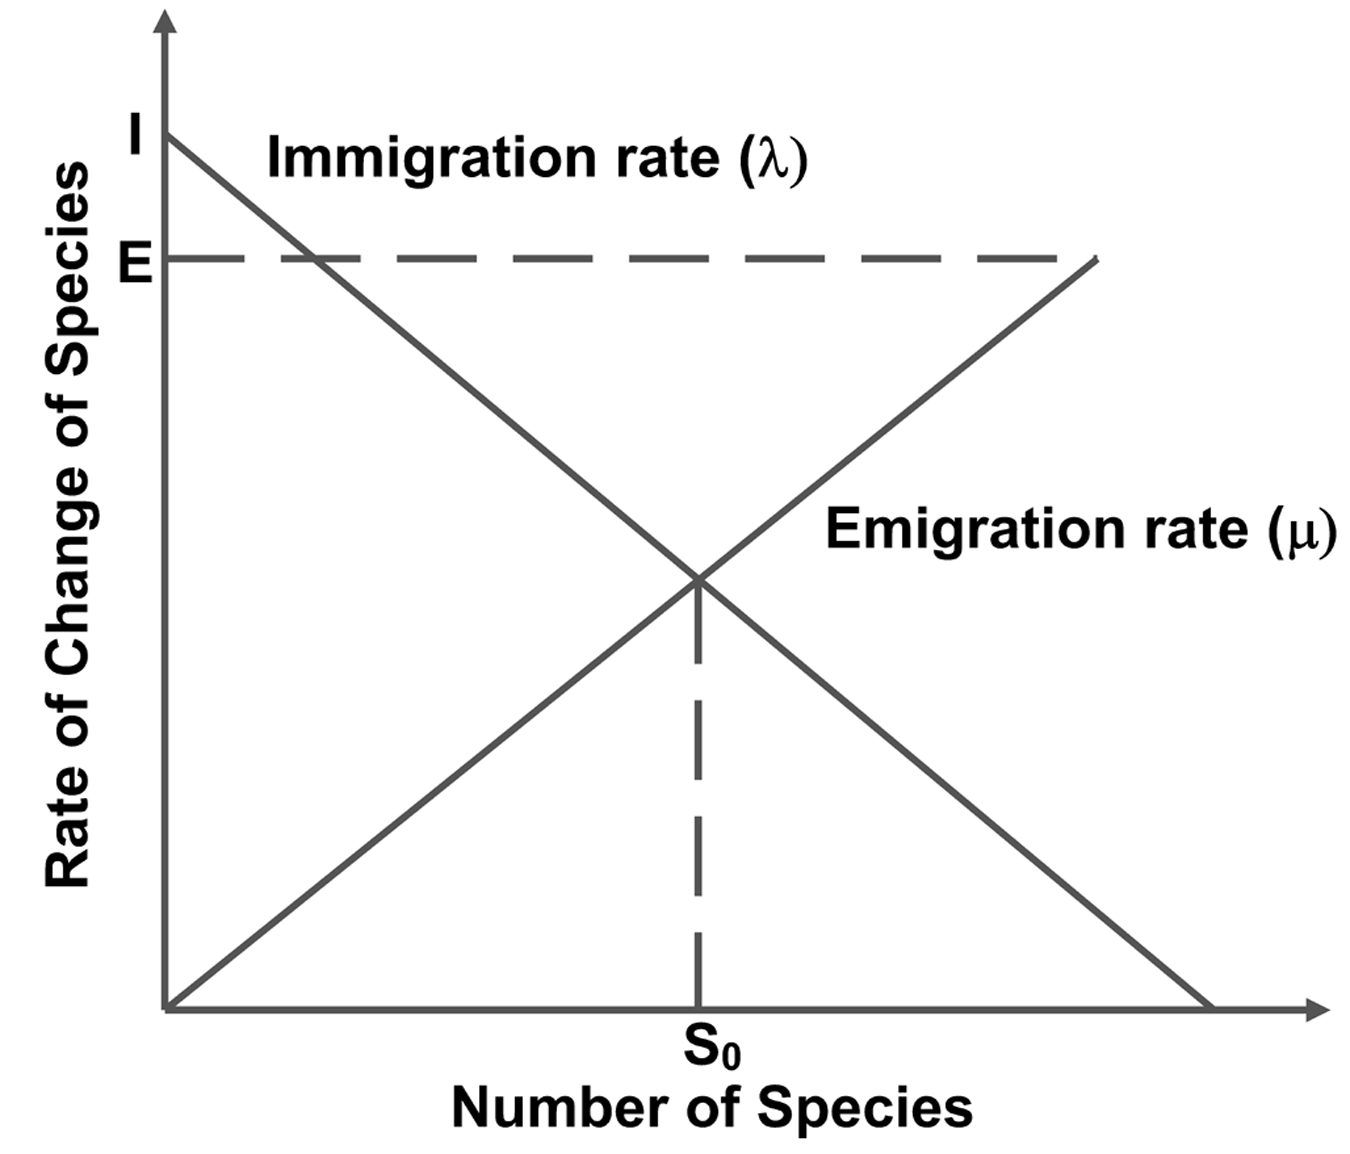
\includegraphics[width=0.38\linewidth]{Equi}
  \caption[ Linear equilibrium model of an ecological system for a single island ]{ \fontsize{12}{10} \selectfont Linear equilibrium model of an ecological system for a single island \cite{Simon2008}}\label{fig:equil}
\end{figure}

BBO initializes the population of individuals in the specified continuous or discrete domain and creates a new population by modifying the existing individuals with the help of three operators, namely elitism, migration, and mutation. BBO follows the elitism property by moving one or more good solutions from the current population to the next generation which perpetuate the quality of solutions in subsequent generations. 


\paragraph{Migration Operator:} Migration is the process in which high ISI solutions, also known as emigrating islands, share its features to low ISI solutions, termed as immigrating islands. Immigrating islands are selected by island modification probability ($P_{modify}$) and immigration rate ($\lambda$) is used to select some of their features which are to be replaced by corresponding features of emigrating islands. Further, the emigration rate ($\mu$) is used by the roulette wheel selection method to select more than one emigrating islands for the same. This process of migration generates new islands that may be selected for the next generation. Algorithm \ref{algo:migration} presents the detailed description of migration process.

\begin{algorithm}
\footnotesize
\caption{\fontsize{10pt}{12pt}\selectfont Migration Operator  \cite{ma2010}}
\label{algo:migration}
\setstretch{1.4}
\begin{algorithmic}
\STATE \textbf{Input:}  A population $P$ of $n$ islands. Each island has $d$ suitability index variables (SIVs).
\STATE Let $P_{modify}$ is the island modification probability.

\STATE \textbf{Output:}  Modified population $P$.

\FOR  {$i= 1\ to\ n$}
  \IF {$rand() < P_{modify}$}
    \STATE    continue;
  \ENDIF
 \FOR  {$j= 1\ to\ d$}

    \IF {$rand() < \lambda_i$}

        \STATE Select emigrating island, $island_k$, according to $\mu_i$ using roulette wheel selection;
           \STATE  $island_i(SIV_j) \leftarrow island_k(SIV_j)$
         
    \ENDIF
\ENDFOR
\ENDFOR
\end{algorithmic}
\end{algorithm}

\paragraph{Mutation Operator:} Mutation is the abrupt extreme alteration in the island due to some calamitous or catastrophic events. It increases the diversity in the islands. In BBO, mutation is performed by replacing some of the SIVs of each island with randomly generated SIVs. These SIVs are chosen on the basis of the mutation rate ($\sigma$) of their corresponding islands. The mutation rate $\sigma_i$ of $i^{th}$ island is calculated by using Eq. (\ref{eq:mrate}).
\begin{equation}\label{eq:mrate}
\sigma_i=mu_{max}*(1-\frac{P_i}{P_{max}} )
\end{equation}
where, ${P_i}$  is the probability of species on $i^{th}$ island at the current time, $mu_{max}$ is the maximum mutation probability, and $P_{max}$  is the maximum probability.  Algorithm \ref{algo:mutation} \cite{ma2010} demonstrates the mutation process of BBO. Moreover, the process of BBO Algorithm has been presented in Algorithm \ref{algo:BBO} \cite{ma2010}.

\begin{algorithm}
\caption{\fontsize{10}{12} \selectfont Mutation Operator \cite{ma2010}}
\label{algo:mutation}
\setstretch{1.4}
\footnotesize

\begin{algorithmic}
\STATE \textbf{Input:} Let population $P$ has $m$ islands ($island_i,\ \ i=1,\ 2,\dots, \ n$) and $\sigma_i$ is the mutation rate of $i^{th}$ island.
\STATE \textbf{Output:} Modified population $P$

\FOR  {$i= 1 \ to\ n$}
     \FOR  {$j= 1\ to\ d$}
        \IF {$\sigma_i > rand()$}
        \STATE Generate a feasible random value R in solution space;
        \STATE $island_i (SIV_j) \leftarrow R$
    \ENDIF
    \ENDFOR
\ENDFOR
\end{algorithmic}
\end{algorithm}

\begin{algorithm}
\caption{\fontsize{10}{12} \selectfont Biogeography-based Optimization \cite{ma2010}}
\label{algo:BBO}
\setstretch{1.4}
\footnotesize
\begin{algorithmic}
\STATE \textbf{Input:} A population $P$ has $n$ islands ($island_i,\ \ i=1,\ 2,\dots, \ n$)
\STATE\textbf{Output:} An optimal island.

 \STATE Measure the value of ISI (fitness) for each island
 \WHILE{stopping condition}
    \STATE  Determine the $\lambda_i$ and $\mu_i$ for each island $island_i$;
    \STATE Perform migration;
    \STATE Perform mutation;
    \STATE Replace one or more worst islands by the previous best islands to perform elitism;
\ENDWHILE
\STATE Select the best island with high ISI.
\end{algorithmic}
\end{algorithm}

%%%%%%%%%survey of BBO 

Sometimes it has been observed that BBO may trap into local optimum and shows slow convergence behavior due to poorly generated population diversity by its mutation and migration operators \cite{pal2017a}. Therefore, researchers have developed different variants of BBO by modifying its migration and mutation operators to enhance the performance. Due et al. \cite{du2009} hybridized BBO with immigration refusal (RE) and evolutionary strategy (ES) to escape from local optimum. Immigration refusal has been used for migration between the individuals while ES has been used to mutate the individuals. Moreover, Gong et al. \cite{gong2010} introduced a real-coded BBO which represents each solution by real parameters in the continuous domain. Further,  to enhance the exploration of the algorithm, they introduced three novel mutation operators, namely levy, Cauchy, and Gaussian. Ma et al. \cite{ma2011}  improved the exploration phase of BBO by introducing a blended migration operator and solved the constrained optimization problem. Further, Lohokare et al. \cite{lohokare2013} introduced a memetic technique to refine the search capability of BBO in which a modified DE has been used with mutation operators to find global optimum in search space.  Moreover, Ma et al. \cite{ma2013} introduced four variants of the migration process, namely BBO with total immigration (BBOTI), BBO with partial immigration (BBOPI), BBO with total emigration (BBOTE), and BBO with partial emigration (BBOPE). The migration process of BBOPI uses immigration rate ($\lambda$) to immigrate an island feature followed by the selection of the emigrating islands. However, BBOTI uses $\lambda$ for immigration of a whole island followed by the selection of the emigrating islands. In contrast to this, BBOTE and BBOPE choose emigrating islands followed by the immigrating island. Therefore, BBOTI and BBOPI use the immigration rate to decide whether migration will occur or not, while BBOTE and BBOPE use the emigration rate for the same. Simon et al. \cite{simon2014} proposed the rotationally invariant migration operator to enhance the performance for non-separable functions. Further, they used a gradient descent operator to overcome the weakness of premature convergence. Moreover, for the real world problems, relying on the constrained boundary, they introduced a global grid search and boundary search to cover the search space systematically. Re-initialization and restart procedures have also been introduced. Gong et al. \cite{gong2010BBO} introduced a hybrid version of BBO and DE in which exploitation is done by BBO while DE performs the exploration to generate an optimal solution. Further, Niu et al. \cite{Niu2014} introduced various mutation strategies for BBO (BBO-M) to maintain the diversity and solutions quality of the population. The modification incorporates the DE with chaos theory in mutation operator. Lim et al. \cite{lim2016} modified the mutation operator of BBO by replacing it with the Tabu search which maintains the population diversity and quality of the population. Further, Al-Roomi et al. \cite{al2016} proposed a novel variant of BBO for improving the exploration capability by hybridizing it with simulated annealing (SA). They used five different cooling strategies and metropolis criteria of SA to select superior migrated islands.  Garg and Deep \cite{Garg2016} proposed a Laplace crossover based BBO, namely LX-BBO, to solve continuous function optimization problems. In addition to above mentioned variants, several other modifications of BBO have also been proposed in literature \cite{saremi2014}, \cite{feng2014}, \cite{zheng2014},\cite{guo2015},  \cite{bansal2016}, \cite{ma2017}. However, most of the variants of BBO either modified migration operator to increase the exploitation capabilities or mutation operator for exploration. In general, migration operator follows the single feature migration property which generates poor performance for non-separable functions \cite{Simon2008}, \cite{gonge2010}, \cite{simon2014}. Moreover, due to poor population diversity, generated by mutation operator increases the chance to converge into local optimum \cite{Simon2008}, \cite{ma2011}, \cite{ma2013}. 


To overcome the above-mentioned limitations, this work introduces two new variants of BBO known as improved BBO (IBBO) and spiral BBO (SBBO) which are discussed in subsequent sections.
 
\subsection{Improved Biogeography-based Optimization} 
  
The existing BBO, as described in the previous section, has two main flaws. The first one is that migration operator follows the single feature migration property i.e., each SIV is handled individually and only a few are updated. This property works well for separable functions in which all the variables are independent. However, a non-separable function contains the inter-dependent variables and that’s why the single feature migration property of BBO algorithms on these functions shows poor performance \cite{simon2014}, \cite{chen2016}.  Secondly, poor population diversity is generated by mutation operator because it replaces some of the selected SIVs of an island with random SIVs. Since, the generated SIVs take random values, the quality of the mutated islands is not guaranteed and quite often solution may trap into local optimum \cite{lim2016}, \cite{ma2011}, \cite{ma2013}. Therefore, in the new improved BBO (IBBO) algorithm, both the migration and mutation operators are modified. The details description of improved operators is provided below. However, the sequence of these operators is similar to the original BBO as described in Algorithm \ref{algo:BBO}.

\subsubsection{Improved Migration Operator}\label{sec: BMO}
The proposed migration operator considers two modifications in the basic migration operator. First, it generates a new island by modifying all the features of the immigrating island, irrespective of original BBO where only limited features are modified. Second, it also uses the best individual along with other islands as emigrating islands while in the original BBO, the best island is not explicitly selected for migration. 

Similar to BBO, the immigrating islands are selected with the help of modification probability $P_{modify}$. If this probability is greater than a random number, then the individual is selected as immigrating islands for modification. Further, the emigrating islands are selected with the help of roulette wheel selection based on $\mu$ i.e., emigration rate. Let each island has $d$ number of SIVs. Now, $d$ number of random numbers are generated. If a generated random number is less than the immigration rate ($\lambda$) then corresponding SIV of immigrating island is replaced by SIV of emigrating island otherwise, selected SIV takes its value from the corresponding best island SIV. This way, all the features of immigrating islands are modified.

In the proposed migration method, the replacement of all SIVs in place of limited SIVs increases exploration capability. Moreover, the use of the best solution increases the chance of generating an optimal result with better convergence rate. Therefore, it also shows efficient results for non-separable functions. The detailed improved migration process is also depicted in Algorithm \ref{algo:Emigration}.


\begin{algorithm}
\caption{\fontsize{10}{12} \selectfont Improved Migration Operator}
\label{algo:Emigration}
\setstretch{1.4}
\footnotesize
\begin{algorithmic}
\STATE \textbf{Input:} A population $P$ of $n$ islands. Each island has $d$ suitability index variables (SIVs).
\STATE Let $P_{modify}$ is the island modification probability.
    \STATE \textbf{Output: } Modified population $P$.

\FOR  {$i= 1\ to\ n$}
  \IF {$rand() < P_{modify}$}
    \STATE    continue;
  \ENDIF
 \FOR  {$j= 1\ to\ d$}
 % \STATE    select $island_i$ according to  $\lambda_i$
    \IF {$rand() < \lambda_i$}
        %\STATE $island_i$ with feature $j$ is selected.
        \STATE Select emigrating island, $island_k$, according to $\mu_i$ using roulette wheel selection;
           \STATE  $island_i(SIV_j) \leftarrow island_k(SIV_j)$
    \ELSE
         \STATE $island_i(SIV_j) \leftarrow island_{best}(SIV_j)$
     
    \ENDIF
\ENDFOR
\ENDFOR
\end{algorithmic}
\end{algorithm}


\subsubsection{Improved Mutation Operator}\label{sec: BMuO}

Mutation is one of the important operators of BBO which is used to create diversity in the population and helps to explore the search space. However, the mutation operator of BBO only modifies some of the SIVs of randomly selected islands due to which it shows poor diversity in the population. 

The proposed method introduces a biased mutation operator based on a random walk and step size. In the biased mutation operator, all the SIVs of randomly selected poor islands are modified. Let $m_i$ is the mutation rate of $i^{th}$ island which is used to select it for mutation. The mutated island for next iteration ($t+1$) is generated by Eq. (\ref{eq:random}).
\begin{equation}\label{eq:random}
island_i(t+1)=island_i(t)+ s_i*r(t), \ i=1, 2,\dots,n
\end{equation}
where, $r \in (0,1)$ is  randomly generated number. Further, $s_i$ denotes the step size of $i^{th}$ island for a random walk. The value of step size ($s$) plays a major role to explore the solution space. The islands with very large step size ($s$) may produce out of bound SIVs which is unacceptable. Moreover, if the step size taken by an island is too small then it will be incapable to explore the search space. Therefore, it is desirable to use a balanced step size for improving the population diversity. The proposed mutation operator obtains the step sizes by differencing the randomly generated permutations of the existing population. 

Let, population $P$ has $n$ islands ($island_i$), as represented by  Eq. (\ref{eq:pop}), and $P^n_k(i)$ represents the randomly generated $k^{th}$ permutation of $i^{th}$ island. The proposed  step size ($s_i$) for  $i^{th}$ island is calculated by Eq. (\ref{eq:stepsize}).
\begin{equation}\label{eq:pop}
P  = \{island_1, island_2, \dots , island_{n-1}, island_n\} \ \ \ 
\end{equation}
\begin{equation}\label{eq:stepsize}
    s_i= P^n_1(i)- P^n_2(i), \ \ \ \ \ i=1,\ 2,\ \dots,n
\end{equation}
The difference between two randomly generated permutations of an island for the current population gives a balanced and random step size. Therefore, the new mutation operator performs random walk with biased behavior which reduces the chances to trap into local optimum and increases population diversity. The detailed process of improved mutation operator is also depicted in Algorithm \ref{algo:Emutation1}.

\begin{algorithm}
\caption{\fontsize{10}{12} \selectfont Improved Mutation Operator}
\label{algo:Emutation1}
\setstretch{1.4}
\footnotesize
\begin{algorithmic}
\STATE \textbf{Input:}  Let population $P$ has $n$ islands ($island_i,\ \ i=1,\ 2,\dots, \ n$) and $\sigma_i$ is the mutation rate of $i^{th}$ island. 
    \STATE \textbf{Output: } Modified population $P$

\FOR  {$i= 1\  to\ n$}
        \IF {$\sigma_i > rand()$}
     \STATE Randomly generate two permutation ($P^n_1(i)$ and $P^n_2(i)$) of $i^{th}$ island;
\STATE $s_i= P^n_1(i)- P^n_2(i)$

        \STATE $island_i(t+1)=island_i(t)+ s_i*r(t)$
    \STATE Check whether $island_i(t+1)$ is feasible or not;
\STATE If not then map to the original bounds;
\ENDIF

\ENDFOR    


\end{algorithmic}
\end{algorithm}

\subsection{Spiral Biogeography-based Optimization}

The existing BBO, as described in Section \ref{ch4:sec:bbo} has poor population diversity which is generated by a mutation operator because it replaces some of the selected SIVs of an island with random SIVs. Since the generated SIVs take only random values, the qualities of the mutated islands are not guaranteed and quite often solution may trap into local optimum \cite{ma2011, lim2016}. Therefore, in the new spiral BBO (SBBO) algorithm, the mutation operator is modified by introducing a spiral search phase in mutation along with random search. The rest of the steps of SBBO remains similar to the original BBO as described in Algorithm \ref{algo:BBO}. 

The new mutation operator generates new SIVs by using two searches; (i) spiral search and (ii) random search, which is explained in the following sections.  

\subsubsection{Spiral Search}

In this phase of mutation operator, some of the SIVs for the new island are searched in a spiral trajectory, as defined by Fermat's spiral function, around the best island so far as shown in Figure \ref{fig:sp} for a two and three-dimensional spaces with radius $r$ and angle $\theta$. In the figure, red and blue spirals correspond to negative and positive $r$ respectively for any given positive value of $\theta$.
\begin{figure}
\centering

     \subfigure[]{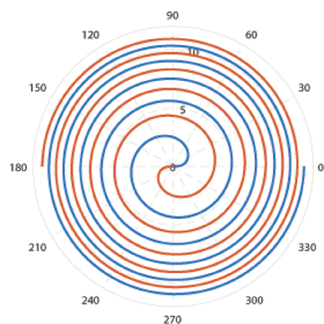
\includegraphics[width=0.42\linewidth]{SpiralPlot}} \hspace{1mm}
       \subfigure[]{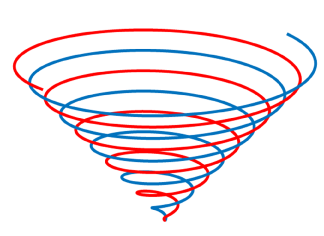
\includegraphics[width=0.5\textwidth]{SpiralPlot3D1}}

  \caption[The Fermat's Spiral Function in 2D and 3D with radius $r$ (0 to 10) angle $\theta$]{\fontsize{10pt}{12pt}\selectfont The Fermat's Spiral Function in (a) 2D and (b) 3D with radius $r$ (0 to 10) and angle $\theta$) }\label{fig:sp}
\end{figure}
The generated spiral trajectory looks like tornadoes and hurricanes. In the BBO, new SIVs are generated using the concept of Fermat's spiral.  Fermat's spiral is a type of Archimedean spiral, also known as a parabolic spiral, and is developed by Fermat et al. \cite{mahoney1994}. Mathematically, it can be  represented by Eq. (\ref{fermat}).
\begin{equation}\label{fermat}
r=\pm\ \theta ^{1/2},
\end{equation}
where, $\theta$ is an angle of rotation and $r$ is a radius of convergence. In polar coordinates, it can be represented as Eq. \ref{fermat1}.
\begin{equation}\label{fermat1}
r^{2}=a^{2}\theta
\end{equation}
here, $a$ is a constant. Further, in a parametric equation, it can be presented as Eq. (\ref{fermat2}) along x-axis. 
\begin{equation}\label{fermat2}
x={\text{sgn}}(a)\cdot |a|\cdot \theta ^{(1/2)}\cdot \cos \theta
\end{equation}
where, $sgn(a)$ corresponds to  the sign function used to extract the sign of a real number. This paper uses the similar movement of species in mutation operator around the best island so far and is defined mathematically by Eq. (\ref{eq:S}).



\begin{equation}\label{eq:S}
 Island_i(t+1)=Island_{Best}(t) + sgn(R_i(t))\cdot|R_i(t)|\cdot l ^{(1/2)}\cdot cos(2*\pi*l) 
\end{equation}
where, $R_i(t)$ is the absolute distance between the best island ($Island_{Best}$) and $i^{th}$ island at $t^{th}$ iteration and $l$ is randomly generated by Eq. (\ref{eq:D11}). 

\begin{equation}\label{eq:D11}
l=  1+ t*rand()/max_{iteration}
\end{equation}


\subsubsection{Random Search}

 The population diversity in BBO can be increased by random search by generating the new SIVs using the randomly selected islands. The mathematical model for random search is given in Eq. (\ref{eq:final2}).

\begin{equation}\label{eq:final2} 
Island_i(t+1)= Island_{random}(t)- R_i(t)
\end{equation}
where, $Island_{random}(t)$ is any random island at iteration $t$, $R_i(t)$ is a residual  distance from the randomly selected island and  is given by Eq. (\ref{eq:D1}).    
\begin{equation}\label{eq:D1}
R_i(t)= \| rand ()* Island_{random} (t)- Island_{i}(t)\|
\end{equation}
here, $rand()$ is a random function for generating the random values between $0$ \& $1$ and $Island_i$ is the $i^{th}$ individual in the population.
The complete improved mutation operator is also presented in Algorithm \ref{algo:Emutation}.
\begin{algorithm}
\caption{\fontsize{10pt}{12pt}\selectfont Improved Mutation Operator}
\label{algo:Emutation}
\setstretch{1.4}
\footnotesize
\begin{algorithmic}
\STATE \textbf{Input:}  Let population $P$ has $n$ islands ($island_i,\ \ i=1,\ 2,\dots, \ n$).
\STATE \textbf{Output: } Modified population $P$
\FOR  {$i= 1\  to\ n$}
        \IF {$rand()<=0.5$}
             \STATE Update the $Island_i$ using Eq. (\ref{eq:S});    
    \ELSE 
        \STATE Select a random island $Island_{random}$;
         \STATE Update the $Island_i$ using Eq. (\ref{eq:final2});
    \ENDIF
\ENDFOR    
\end{algorithmic}
\end{algorithm} 


\section{Optimal Codebook Construction}
The new variant of BBO, namely IBBO and SBBO are used to generate the optimal visual words in the BOF method. The BOF method is modified by introducing a new clustering method in place of K-means. The new clustering method uses IBBO/SBBO to find optimal cluster centers. The nearby features of the cluster centers are considered as the optimal visual words. The complete process of the modified BOF method is described below.

\begin{enumerate}
\item  The $D$-dimensional feature vectors are extracted from the collection of histopathological images.

\item Optimal  set of visual words are computed using the following IBBO/SBBO based clustering methods.
\begin{enumerate}
\item Let the set $F$ of local features are $\{f_1, f_2, \cdots, f_N\}$ where $f_n \in \mathbb{R}^D$. Apply K-means on the set $F$ to find the K cluster centers \{$c_1, c_2, \cdots, c_K$\} where, $c_k \in \mathbb{R}^D$. 

\item Initialize the population of $M$ islands. Each island is a vector of  $K$ features that are nearby to the centroids returned K-means.  

\item Calculate the fitness of each island by considering the following objective function

\begin{equation}\label{eq:fitness} 
Minimize  \ \ \delta(f_m, c_k)   =  \sum_{i=1}^N \sum_{j=1}^K \parallel f_m - c_k \parallel ^2
\end{equation}
 where, $\delta$ represents the compactness of the clusters and the objective is to minimize the compactness for better clustering.
 
 \item Determine better solutions to perform elitism. 

\item Improve the quality of the population by performing migration and mutation operators of IBBO/SBBO.

\item Repeat Steps (c) to (e) until the termination criteria are not achieved.

\item Determine the best island in the last iteration.

\end{enumerate}

\item The nearby features of the best island are considered as visual words.

\item Each image is encoded by the optimal set of visual words in the form of a histogram.

\item The encoded histograms along with the image annotations are used to train the SVM classifier. Finally, the trained SVM classifier is tested on the validation dataset.  

\end{enumerate}




\section{Experimental Results}\label{sec:exp}

This section presents the results of IBBO and SBBO methods along with the IBBO/SBBO  based BOF method for histopathological image classification. Section \ref{ch4:subsec:results1} analyzes the effectiveness of IBBO and SBBO on various benchmark functions while experimental results of histopathological image classification on ADL and Blue histology datasets are presented in Section \ref{ch4:subsec:results2}.



\subsection{Performance Analysis of IBBO and SBBO}\label{ch4:subsec:results1}
The performance of newly introduced IBBO and SBBO  have been analyzed on $20$ representative benchmark functions as listed in Table \ref{tab:BenchmarkFunctions} \cite{yang2014} \cite{Simon2013} \cite{jamil2013}  and $29$ bound-constrained CEC 2017 benchmark problems  \cite{wu2016} as depicted in Table \ref{tab:CEC2017}. The performance has been evaluated and statistically analyzed using three performance parameters, namely mean fitness value, rank value using Friedman test, and convergence. 


\begin{table}[t]
\scriptsize
\centering
\caption[Standard benchmark functions]{\fontsize{10}{12} \selectfont Summary of standard benchmark problems}
\renewcommand{\arraystretch}{1.2}
 \begin{tabular}{p{0.3in} p{1.2in}  p{0.9in} p{0.8in} p{1.5in} p{0.6in}}
    \hline
\textbf{Sr. No.}  &\textbf{Function Name}    &                \textbf{Range }     & \textbf{Optimal Value} &\textbf{Optimal Position Values }&\textbf{Category}\\
\hline

1.    &    Ackley    &        [-35 to 35]    &     0    &     (0,\dots,0) & MM,\ NS\\
2.    &    Alpine    &        [-10 to 10]     &    0    &     (0,\dots,0)& MM,\ S\\
3.    &    Brown    &    [-5 to 5] &    0    &    (0,\dots,0)& UM,\ NS\\
4.    &    Levy    &    [-10 to 10]     &     0    &     (1,1,,\dots,1)& MM\\
5.    &    New Schwefel    &        [-500 to 500]     &    0    &     (420.9687,..., 420.9687)& MM\\
6.    &    Pathological    &        [-100 to 100]     &    0    &    (0,\dots,0)& MM,\ NS\\
7.    &    Penalty1    &         [-50 to 50]    &     0    &    (1,1,\dots,1)    & MM,\ NS\\
8.    &    Penalty2    &         [-50 - 50]        & 0    &      (1,1,\dots,1) &MM,\ NS\\
9.    &    Powell's First Singular    &        [-4 - 5]    &    0     &    (0,0,\dots,0)& UM,\ NS\\
10.    &    Powell's Second Singular    &        [-4 - 5]    &    0    &     (0,0,\dots,0) & UM,\ NS\\
11.    &    Powell Sum    &        [-1 - 1]    &    0     &    (0,0,\dots,0)    & UM,\ S\\
12.    &    Quartic    &        [-1.28 - 1.28]    &    0    &    (0,0,\dots,0)    & UM,\ S\\
13.    &    Rastrigin    &        [-5.12 - 5.12]    &    0    &     (0,0,\dots,0)    & MM\\
14.    &    Rotated Hyper-Ellipsoid    &        [-65.536 - 65.536]     &    0    &     (0,0,\dots,0)    & UM\\
15.    &    Schwefel    &        [-512 - 512]    &    -12965.5     &         (420.9687,..., 420.9687)& MM,\ S\\
16.    &    Schwefel3    &    [-10 - 10]     &     0    &     (0,0,\dots,0& MM,\ NS \\
17.    &    Sphere    &        [-5.12 - 5.12]    &    0    &(0,0,\dots,0)    & UM,\ S\\
18. &    Step    &        [-100 - 100]    &     0    &     (0,\dots,0)& UM,\ S\\
19.    &    Sum Squares    &        [-10 - 10]     &    0 &    (0,0,\dots,0)    & UM,\ S\\
20.    &    Trigonometric    &        [0 - $\pi$]    &     0    &     (0,0,\dots,0& MM,\ NS \\
\hline
\end{tabular}
\label{tab:BenchmarkFunctions}
\end{table}


\begin{table}[t]
\scriptsize
\caption[Overview of CEC 2017 benchmark problems]{\fontsize{10}{12} \selectfont Overview of CEC 2017 benchmark problems}
\centering
\renewcommand{\arraystretch}{1.2}
\begin{tabular}{p{1in}   p{2in}   p{0.8in} p{0.9in}}
    \hline
\textbf{S.No.}& \textbf{Function}  &  \textbf{Optimal Value } &\textbf{Characteristic}\\
\hline
$C_1$ & SR Bent Cigar Function & 100 &   \\
$C_2$ & SR Sum of Different Power Function & 200 &Unimodal \\
$C_3$ & SR Zakharov Function & 300 &  \\ 
\hline
 $C_4$& SR Rosenbrock’s Function & 400 &\\ 
 $C_5$& SR Rastrigin’s Function & 500 & \\ 
 $C_6$& SR Expanded Scaffer’s F6 Function & 600 & \\ 
 $C_7$& SR Lunacek B\_Rastrigin Function & 700 &  Multi-modal \\ 
$C_8$& SR Non-Continuous Rastrigin’s Function & 800 & \\  
$C_9$& SR Levy Function & 900 & \\
$C_{10}$ & SR Schwefel’s Function & 1000 &   \\
\hline
$C_{11}$ & HF 1  & 1100 &  \\
 $C_{12}$& HF  2  & 1200 & \\
 $C_{13}$& HF  3  & 1300 &  \\
 $C_{14}$& HF  4  & 1400 & \\
 $C_{15}$& HF  5 & 1500 &  Hybrid\\
 $C_{16}$& HF  6 & 1600 & \\
 $C_{17}$& HF  6 & 1700 & \\
 $C_{18}$& HF  6  & 1800 & \\
 $C_{19}$& HF  6  & 1900 & \\
 $C_{20}$& HF  6  & 2000 &  \\
\hline
$C_{21}$ & CF 1 (N=3) & 2100 &  \\
 $C_{22}$& CF 2 (N=3) & 2200 & \\
 $C_{23}$& CF 3 (N=4) & 2300 & \\
 $C_{24}$& CF 4 (N=4) & 2400 & \\
 $C_{25}$& CF 5 (N=5) & 2500 & Composition \\
 $C_{26}$& CF 6 (N=5) & 2600 & \\
 $C_{27}$& CF 7 (N=6) & 2700 & \\
 $C_{28}$& CF 8 (N=6) & 2800 & \\
 $C_{29}$& CF 9 (N=3) & 2900 & \\
 $C_{30}$& CF 10 (N=3) & 3000 &  \\
\hline
\end{tabular}


SR: Shifted and Rotated; HF: Hybrid Function; CF: Composite Function
\label{tab:CEC2017}
\end{table}

Each considered benchmark function of Table \ref{tab:BenchmarkFunctions}  belongs to either unimodal (UM) or multi-modal (MM) class and/or separable (S) or non-separable (NS) class.  Table \ref{tab:BenchmarkFunctions} also depicts the search space, optimal value, category, the optimal solution value for each benchmark function. Moreover, the functions of CEC $2017$ contain novel basic problems, composing test problems, rotated trap problems, graded level linkages, and many other problems. These benchmark problems show several novel features like composing $3$, $4$, $5$, and $6$ test problems by considering features from various problems and rotated trap problems \cite{brest2017single}. In CEC $2017$, $30$ problems were defined in which three problems are unimodal ($C_1$-$C_3$), seven problems are multi-modal ( $C_4$-$C_{10}$), ten problems are hybrid ($C_{11}$-$C_{20}$), and ten are composition based problems ($C_{21}$-$C_{30}$). Every function contains the search space $[-100,100]^D$ where $D$ is the dimension. Function $C_2$ is excluded from the competition due to its unstable behavior. Figure \ref{fig:fplot} shows the 3D map of two multi-modal ($C_5$ and $C_6$) and two composition ($C_{22}$ and $C_{28}$) functions respectively. From the figure, it can be visualized that functions $C_5$ and $C_6$ contain multiple local optima and global optimum is not near to the second better local optimum. Further, $C_{22}$ and $C_{28}$ have different properties around different local optima due to its composite nature. 
\begin{figure}
    \centering
\subfigure[]{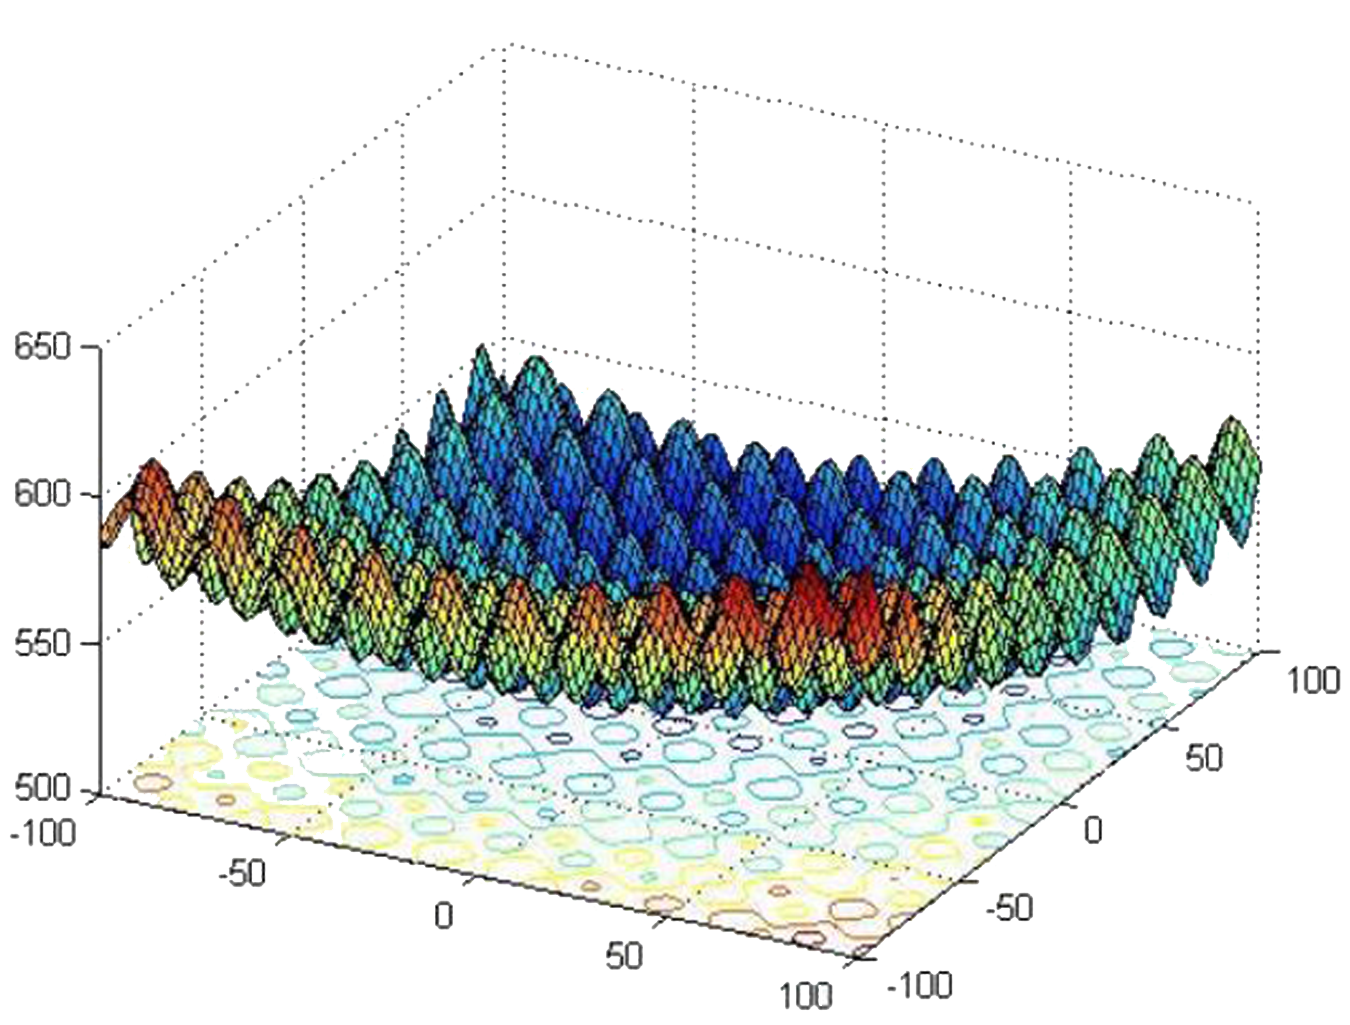
\includegraphics[width=0.33\textwidth]{F5}} 
\subfigure[]{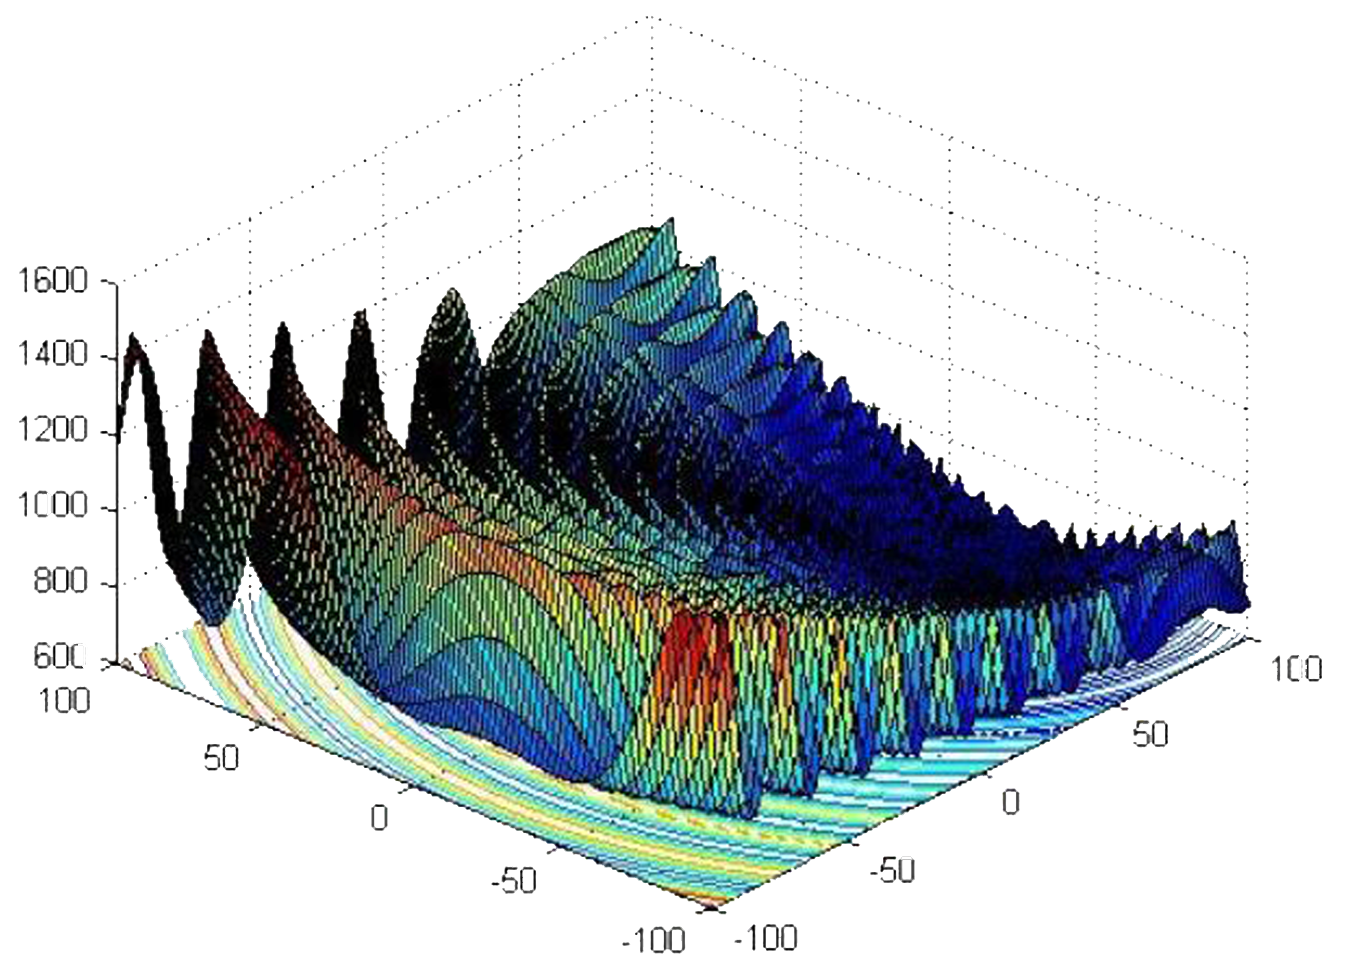
\includegraphics[width=0.33\textwidth]{F6}}
\subfigure[]{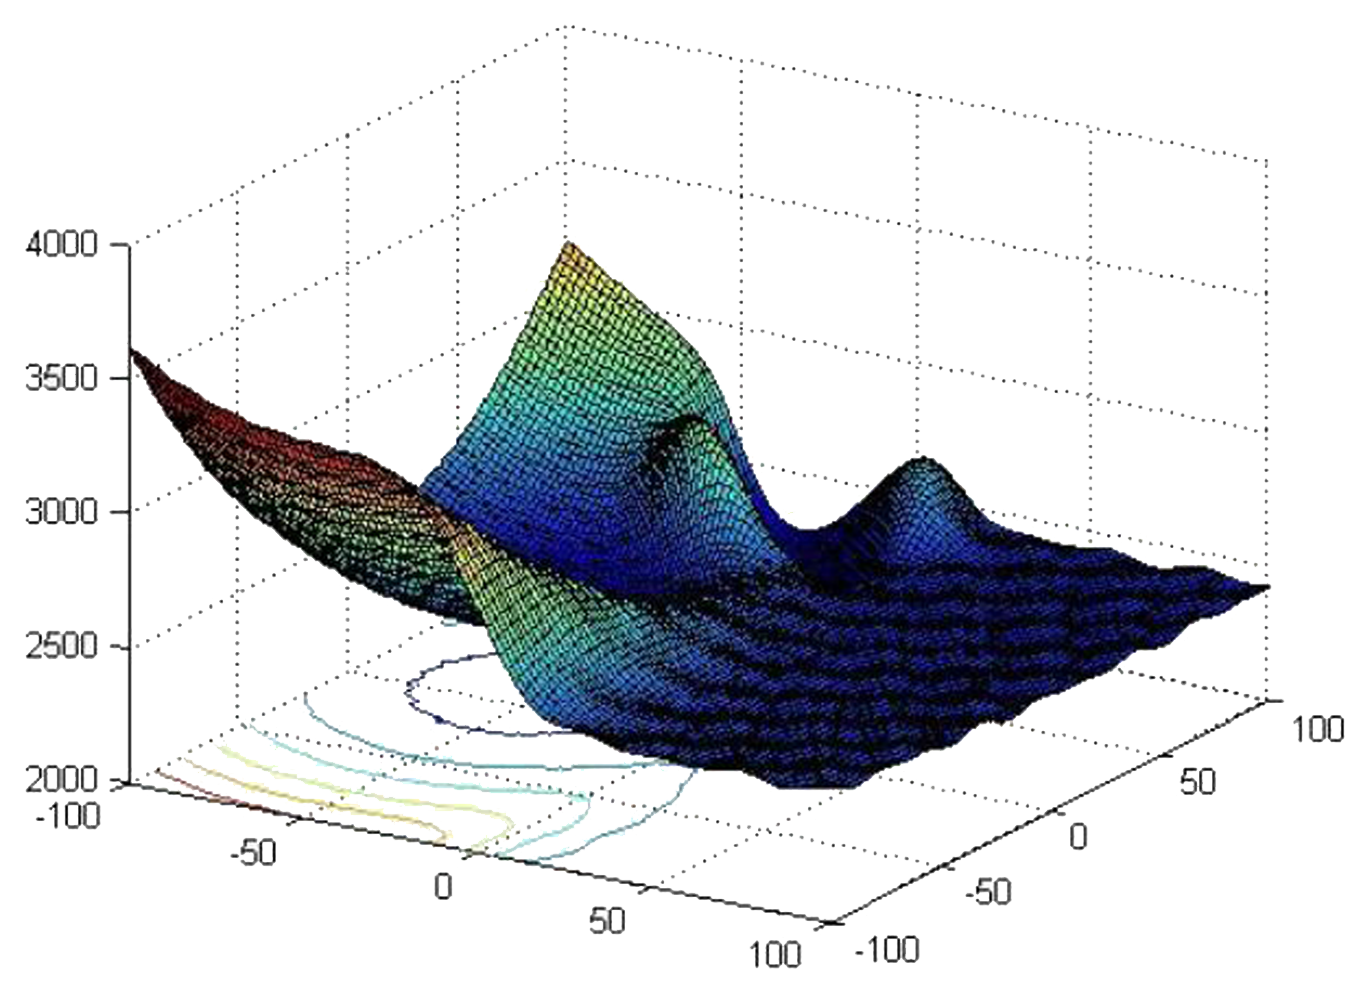
\includegraphics[width=0.33\textwidth]{F22}}
\subfigure[]{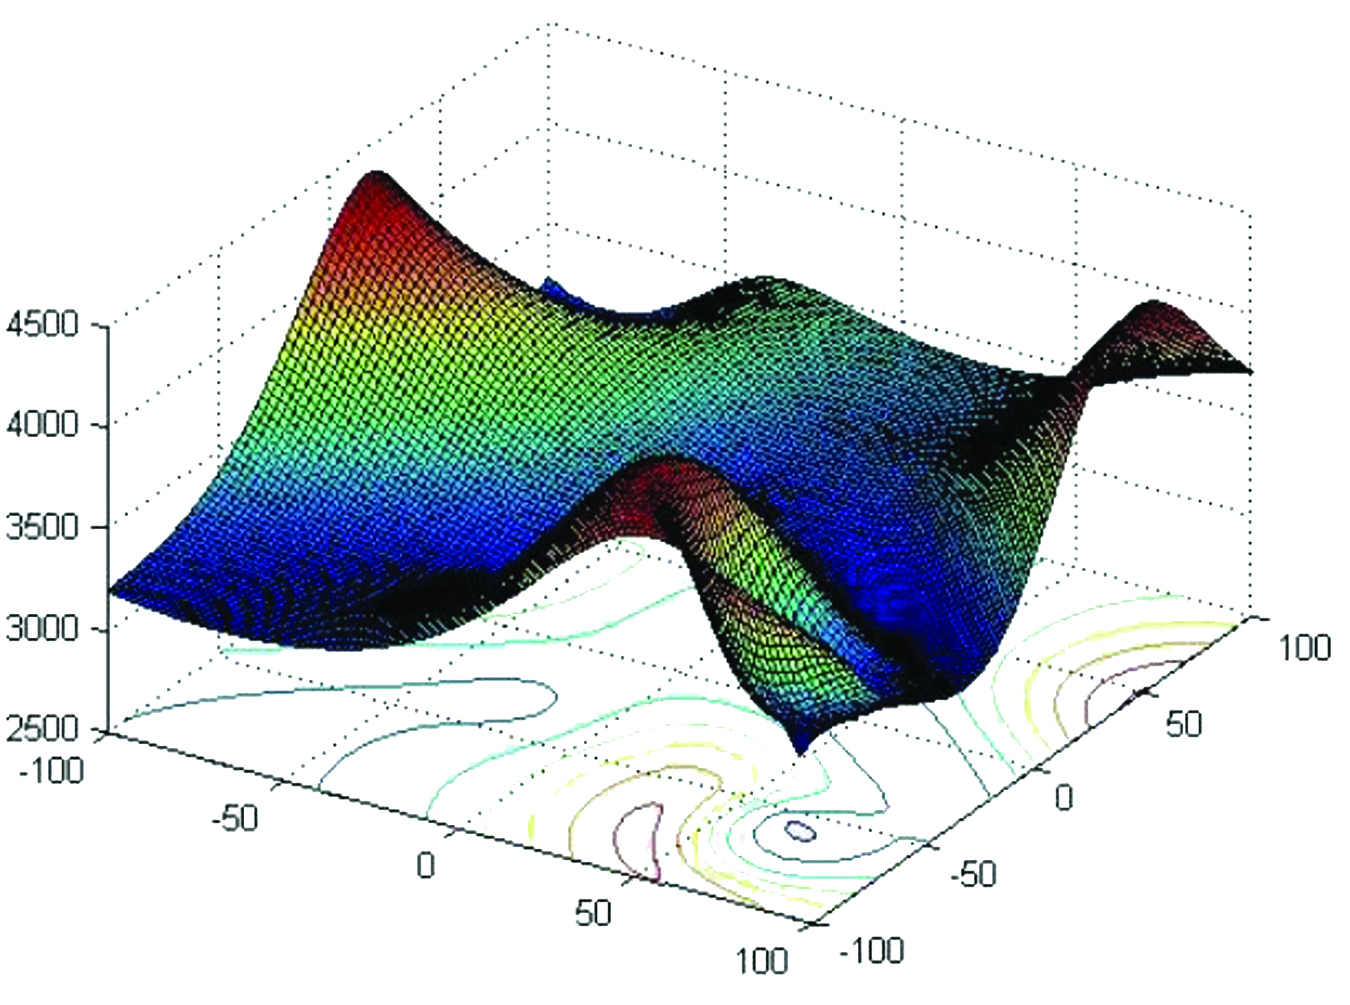
\includegraphics[width=0.33\textwidth]{F28}}
 \caption[3D map for multi-modal and composition based benchmark problems]{\fontsize{10pt}{12pt}\selectfont  3D map for (a) $C_5$, (b) $C_6$,  (c) $C_{22}$, and (d) $C_{28}$  benchmark problems of CEC 2017 \cite{wu2016}}
\label{fig:fplot}
\end{figure}

For the comparative analysis of SBBO and IBBO, one variant of EA, namely LSHADE (differential evolution based on success history and population size) \cite{Mohamed2017}, two variants of BBO, namely BBO-M \cite{Niu2014}, LX-BBO \cite{Garg2016}, and four variants of swarm-based approaches, namely  SSA \cite{Mirjalili2017},  GWO (grey wolf optimizer) \cite{mirjalili2014}, ckGSA (chaotic GSA) \cite{mittal2016}, and WOA (whale optimization Algorithm ) \cite{mirjalili2016} have been simulated along with the BBO algorithm. The parameter settings of all the considered algorithms have been set according to their literature except population size ($N$),  number of dimensions ($D$), and  number of iterations ($itr$) which are kept to $100$, $50$, and $1000$ respectively. To minimize the interference, the simulations have been executed $30$ times.  


Table \ref{tab:mean1} \& \ref{tab:mean2} depict the mean fitness values for $30$, $60$, and $90$ dimensions, generated by each existing and new methods  on standard benchmark functions. Table \ref{tab:mean1} shows the comparative view for the functions $F_1$ to $F_{10}$ while, $F_{11}$ to $F_{20}$ are depicted in Table \ref{tab:mean2}. In the tables, bold entries indicate the best results. It is envisioned from the table that IBBO and SBBO perform much superior to the existing methods, however between the two, SBBO performs the best. Moreover, Table \ref{tab:mean3} depicts the comparison of the IBBO and SBBO with considered algorithms on unimodal, multi-modal, hybrid, and composite benchmark problems of CEC 2017 in terms of mean fitness values. From the table, it can be stated that mean fitness values returned by SBBO are better than the other algorithms for $23$ problems out of $29$. For the unimodal problem $C_1$, BBO-M shows better mean fitness value. However, for the same problem, the second best mean fitness value is returned by SBBO. Similarly, for the multi-modal and composite benchmark problems, SBBO outperforms on all the problems.  Moreover, for hybrid benchmark problems, SBBO shows better results except $C_{11}$, $C_{13}$, $C_{15}$, and $C_{19}$ where BBO-M and LX-BBO perform better. From Table \ref{tab:mean3}, it can be seen that IBBO does not perform adequately for CEC 2017 functions

\begin{sidewaystable}
\scriptsize
\caption[Mean fitness values returned by IBBO, SBBO and other methods on the standard benchmark functions ($F_1$ to $F_{10}$)]{\fontsize{10}{12} \selectfont Mean fitness values returned by IBBO, SBBO and other methods on the standard benchmark functions ($F_1$ to $F_{10}$) }
\begin{center}
\renewcommand{\arraystretch}{1.3}
\begin{tabular}{p{0.3in} | p{0.4in} | p{0.6in} |  p{0.6in} |  p{0.6in}|  p{0.6in} |  p{0.6in} | p{0.6in} |  p{0.6in} | p{0.6in} |  p{0.6in} |  p{0.6in}}
 \hline
\textbf{Func.}     &     \textbf{Dims.}     &     \textbf{BBO}     &     \textbf{BBO-M} &     \textbf{GWO}     &     \textbf{ckGSA}     &     \textbf{LXBBO}     &     \textbf{WOA}     &    \textbf{LSHADE}     &     \textbf{SSA}     &     \textbf{IBBO}     &    \textbf{SBBO} \\
\hline
&    30    &{    1.38e-01    }&    1.260    &    1.440    &    1.300    &    4.71e-01    &    4.24e-01    &    1.98e-01    &    1.78e-01    &    \textbf{    0    }&    \textbf{    0    }\\
F1    &    60    &{    4.96e-01    }&    1.930    &    3.110    &    2.800    &    8.26e-01    &    7.43e-01    &    6.34e-01    &    5.71e-01    &    {    3.45e-03    }&    \textbf{    2.42e-03    }\\
    &    90    &{    8.84e-01    }&    2.490    &    3.780    &    3.400    &    1.070    &    9.63e-01    &    1.090    &    9.81e-01    &    {    8.63e-02    }&    \textbf{    6.04e-02    }\\
\hline                                                                                                            
    &    30    &    5.02e-04    &    2.69e-03    &    8.50e-01    &    7.65e-01    &    9.76e-03    &    8.78e-03    &    4.99e-04    &{    4.49e-04    }&    \textbf{    0    }&    \textbf{    0    }\\
F2    &    60    &{    5.10e-01    }&    3.04e01    &    3.12e01    &    2.81e01    &    1.820    &    1.640    &    1.140    &    1.030    &    \textbf{    0    }&    \textbf{    0    }\\
    &    90    &{    3.840    }&    8.49e01    &    5.81e01    &    5.23e01    &    5.260    &    4.730    &    7.480    &    6.730    &    \textbf{    0    }&    \textbf{    0    }\\
    \hline                                                                                                        
    &    30    &\textbf{    0    }&    5.60e-14    &\textbf{    0    }&\textbf{    0    }&    5.63e-03    &    5.07e-03    &\textbf{    0}    &\textbf{    0}&    \textbf{0}&    \textbf{0}\\
F3    &    60    &    4.84e-02    &    1.46e-03    &\textbf{    0    }&\textbf{    0    }&    4.050    &    3.650    &    1.77e-01    &    1.59e-01    &    \textbf{    0    }&    \textbf{    0    }\\
    &    90    &    1.880    &    9.77e-01    &    7.79e-02    &{    7.01e-02    }&    2.26e01    &    2.03e01    &    4.490    &    4.040    &    \textbf{    0    }&    \textbf{    0    }\\
\hline
    &    30    &    2.45e-03    &    1.06e-10    &\textbf{    0    }&\textbf{    0    }&    8.00e-03    &    7.20e-03    &    6.08e-04    &    5.47e-04    &    \textbf{    0    }&    \textbf{    0    }\\
F4    &    60    &    9.95e-01    &    1.660    &    1.60e01    &    1.44e01    &    1.020    &{    9.18e-01    }&    1.710    &    1.540    &    \textbf{    0    }&    \textbf{    0    }\\
    &    90    &    4.980    &    5.43e01    &    5.94e01    &    5.35e01    &    2.750    &{    2.480    }&    9.460    &    8.510    &    \textbf{    0    }&    \textbf{    0    }\\        
    \hline                                        
    &    30    &{    1.25e01    }&    5.40e02    &    2.12e02    &    1.91e02    &    9.95e02    &    8.96e02    &    1.77e01    &    1.59e01    &    {    3.540    }&    \textbf{    2.480    }\\
F5        &60    &    2.09e02    &    1.50e04    &    8.81e03    &    7.93e03    &    4.55e03    &    4.10e03    &    5.51e02    &    4.96e02    &    {    4.14e01    }&    \textbf{    2.90e01    }\\
    &    90    &    8.85e02    &    2.54e04    &    1.72e04    &    1.55e04    &    8.73e03    &    7.86e03    &    2.54e03    &    2.29e03    &    {    1.57e02    }&    {    1.10e02    }\\
\hline
    &    30    &{    2.670    }&    2.980    &    4.410    &    3.970    &    5.050    &    4.550    &    2.880    &{    2.590    }&            2.760    &    \textbf{    1.930    }\\
F6    &    60    &    7.560    &{    6.860    }&    1.33e01    &    1.20e01    &    1.29e01    &    1.16e01    &    8.500    &    7.650    &    {    6.830    }&    \textbf{    4.780    }\\
    &    90    &{    1.45e01    }&    2.05e01    &    2.34e01    &    2.11e01    &    2.19e01    &    1.97e01    &    1.70e01    &    1.53e01    &    {    1.12e01    }&    \textbf{    7.840    }\\            
\hline                                    
    &    30    &    1.90e-03    &{    3.33e-10    }&    1.150    &    1.040    &    2.33e-02    &    2.10e-02    &    1.10e-02    &    9.90e-03    &    \textbf{    0    }&    \textbf{    0    }\\
F7    &    60    &    8.820    &    3.70e01    &    1.11e01    &    9.990    &    2.840    &{    2.560    }&    1.50e01    &    1.35e01    &    {    1.05e-02    }&    \textbf{    7.35e-03    }\\
    &    90    &    6.07e01    &    3.71e06    &    4.46e01    &    4.01e01    &    9.240    &{    8.320    }&    3.51e03    &    3.16e03    &    {    1.17e-01    }&    \textbf{    8.19e-02    }\\        
\hline                                                
    &    30    &    5.51e-01    &{    2.42e-09    }&    2.920    &    2.630    &    1.650    &    1.490    &    9.54e-01    &    8.59e-01    &    \textbf{    0    }&    \textbf{    0    }\\
F8    &    60    &    6.85e01    &    9.92e01    &    1.46e02    &    1.31e02    &    1.38e01    &{    1.24e01    }&    2.79e03    &    2.51e03    &    {    1.77e-01    }&    \textbf{    1.24e-01    }\\
    &    90    &    6.94e04    &    8.24e06    &    1.49e06    &    1.34e06    &    4.46e01    &{    4.01e01    }&    4.37e05    &    3.93e05    &    {    1.390    }&    \textbf{    9.73e-01    }\\                                                        \hline            
    &    30    &    7.17e-01    &    2.17e01    &    5.420    &    4.880    &{    8.40e-02    }&\textbf{    7.56e-02    }&    1.300    &    1.170    &            4.77e-01    &    {    3.34e-01    }\\
F9    &    60    &    4.31e01    &    5.13e03    &    5.97e01    &    5.37e01    &    1.45e01    &{    1.31e01    }&    1.24e02    &    1.12e02    &    {    5.100    }&    \textbf{    3.570    }\\
    &    90    &    2.39e02    &    1.79e04    &    2.64e02    &    2.38e02    &    4.09e01    &{    3.68e01    }&    4.61e02    &    4.15e02    &    {    1.75e01    }&    \textbf{    1.23e01    }\\
\hline                                                                                                    
    &    30    &    8.40e-03    &    8.45e-06    &\textbf{    0    }&\textbf{    0    }&    2.140    &    1.930    &    3.15e- 03    &    3.00e-03    &    \textbf{    0    }&    \textbf{    0    }\\
F10    &    60    &    3.63e01    &{    4.080    }&    1.43e02    &    1.29e02    &    7.14e01    &    6.43e01    &    9.40e01    &    8.46e01    &    \textbf{    0    }&    \textbf{    0}\\
    &    90    &    5.97e02    &    3.74e03    &    1.02e04    &    9.18e03    &    3.26e02    &    2.93e02    &    1.55e03    &    1.40e03    &    \textbf{    0}&    \textbf{    0    }\\
\hline            

\end{tabular}
\end{center}
\label{tab:mean1}
\end{sidewaystable}


\begin{sidewaystable}
\scriptsize
\caption[Mean fitness values returned by IBBO, SBBO and other methods on the standard benchmark functions ($F_{11}$ to $F_{20}$) ]{\fontsize{10}{12} \selectfont Mean fitness values returned by IBBO, SBBO and other methods on the standard benchmark functions ($F_{11}$ to $F_{20}$) }
\begin{center}
\renewcommand{\arraystretch}{1.3}
\begin{tabular}{p{0.3in} | p{0.4in} | p{0.6in} |  p{0.6in} |  p{0.6in}|  p{0.6in} |  p{0.6in} | p{0.6in} |  p{0.6in} | p{0.6in} |  p{0.6in} |  p{0.6in}}
  
\hline\textbf{Func.}     &     \textbf{Dims.}     &     \textbf{BBO}     &     \textbf{BBO-M} &     \textbf{GWO}     &     \textbf{ckGSA}     &     \textbf{LXBBO}     &     \textbf{WOA}     &    \textbf{LSHADE}     &     \textbf{SSA}     &     \textbf{IBBO}     &    \textbf{SBBO} \\
\hline
    &    30    &\textbf{    0    }&    4.44e-25    &\textbf{    0    }&\textbf{    0    }&    4.54e-57    &    4.09e-57    &\textbf{    0    }&\textbf{    0    }&    \textbf{    0    }&    \textbf{    0    }\\
F11    &    60    &    9.22e-38    &    1.78e-07    &\textbf{    0    }&\textbf{    0    }&    1.13e-24    &    1.02e-24    &    4.97e-29    &    4.47e-29    &    \textbf{    0    }&    \textbf{    0    }\\
    &    90    &    4.33e-12    &    3.55e-02    &\textbf{    0    }&\textbf{    0    }&    2.28e-21    &    2.05e-21    &    6.66e-15    &    5.99e-15    &    \textbf{    0    }&    \textbf{    0    }\\
\hline                                                                                                            
    &    30    &\textbf{    0    }&    5.40e-27    &\textbf{    0    }&\textbf{    0    }&    4.56e-15    &    4.10e-15    &\textbf{    0    }&\textbf{    0    }&    \textbf{    0    }&    \textbf{    0    }\\
F12    &    60    &    4.81e-04    &    3.36e-04    &\textbf{    0    }&\textbf{    0    }&    5.68e-05    &    5.11e-05    &    5.63e-04    &    5.07e-04    &    \textbf{    0    }&    \textbf{    0    }\\
    &    90    &    9.53e-02    &    1.510    &\textbf{    0    }&\textbf{    0    }&    2.03e-03    &    1.83e-03    &    1.70e-01    &    1.53e-01    &    \textbf{    0    }&    \textbf{    0    }\\
\hline                                                                                                            
    &    30    &\textbf{    0    }&    1.26e02    &    4.530    &    4.080    &    1.220    &    1.100    &\textbf{    0    }&\textbf{    0    }&    \textbf{    0    }&    \textbf{    0    }\\
F13    &    60    &{    1.600    }&    4.48e02    &    7.52e01    &    6.77e01    &    1.75e01    &    1.58e01    &    4.920    &    4.430    &    \textbf{    0    }&    \textbf{    0    }\\
    &    90    &{    2.30e01    }&    8.33e02    &    2.28e02    &    2.05e02    &    5.40e01    &    4.86e01    &    3.13e01    &    2.82e01    &    \textbf{    0    }&    \textbf{    0    }\\
\hline                                                                                                            
    &    30    &    4.47e01    &\textbf{    2.23e-37    }&    1.11e03    &    9.99e02    &    1.48e02    &    1.33e02    &    9.18e01    &    8.26e01    &    {    6.30e-01    }&    {    4.41e-01    }\\
F14    &    60    &    3.21e03    &\textbf{    1.06e01    }&    6.46e04    &    5.81e04    &    2.25e03    &    2.03e03    &    6.81e03    &    6.13e03    &            6.71e01    &    {    4.70e01    }\\
    &    90    &    2.80e04    &    9.34e03    &    3.23e05    &    2.91e05    &    8.85e03    &    7.97e03    &    5.44e04    &    4.90e04    &    {    7.42e02    }&    {    5.19e02    }\\
\hline                                                                                                            
    &    30    &    1.20e02    &    1.76e03    &    5.54e02    &    4.99e02    &    9.25e01    &    8.33e01    &    2.21e01    &{    1.99e01    }&    \textbf{    5.090    }&    \textbf{    3.560    }\\
F15    &    60    &    2.10e02    &    8.05e03    &    3.96e03    &    3.56e03    &    4.16e03    &    3.74e03    &    5.11e02    &    4.60e02    &    \textbf{    3.05e01    }&    \textbf{    2.14e01    }\\
    &    90    &    1.18e03    &    1.73e04    &    7.74e03    &    6.97e03    &    9.43e03    &    8.49e03    &    2.42e03    &    2.18e03    &    {    1.41e02    }&    {    9.87e01    }\\
\hline                                                                                                            
    &    30    &\textbf{    0    }&    2.46e-06    &    2.11e01    &    1.90e01    &    7.44e-02    &    6.70e-02    &    5.28e-03    &    4.75e-03    &    \textbf{    0    }&    \textbf{    0    }\\
F16    &    60    &    2.000    &{    7.31e-01    }&    9.94e01    &    8.95e01    &    5.460    &    4.910    &    4.070    &    3.660    &    \textbf{    0    }&    \textbf{    0    }\\
    &    90    &{    1.08e01    }&    3.00e01    &    2.22e02    &    2.00e02    &    1.46e01    &    1.31e01    &    1.98e01    &    1.78e01    &    \textbf{    0    }&    \textbf{    0    }\\
\hline                                                                                                            
    &    30    &    9.62e-04    &{    6.11e-09    }&    1.820    &    1.640    &    1.510    &    1.360    &    1.40e-01    &    1.26e-01    &    \textbf{    0    }&    \textbf{    0    }\\
F17    &    60    &    1.93e-01    &{    3.34e-03    }&    2.18e01    &    1.96e01    &    2.49e-01    &    2.24e-01    &    7.73e-01    &    6.96e-01    &    \textbf{    0    }&    \textbf{    0    }\\
    &    90    &    2.960    &    2.060    &    7.60e01    &    6.84e01    &    1.060    &{    9.54e-01    }&    7.770    &    6.990    &    \textbf{    0    }&    \textbf{    0    }\\
\hline                                                                                                            
    &    30    &    3.00e-01    &\textbf{    0    }&    1.13e02    &    1.02e02    &    1.900    &    1.710    &    2.400    &    2.160    &    {    2.00e-01    }&    {    1.40e-01    }\\
F18    &    60    &    2.87e01    &\textbf{    0    }&    5.10e02    &    4.59e02    &    4.25e01    &    3.83e01    &    5.78e01    &    5.20e01    &    {    6.700    }&    {    4.690    }\\
    &    90    &    1.28e02    &    1.01e02    &    1.05e03    &    9.45e02    &    1.06e02    &    9.54e01    &    2.56e02    &    2.30e02    &    {    2.34e01    }&    \textbf{    1.64e01    }\\
\hline                                                                                                            
    &    30    &    9.63e-03    &{    6.33e-10    }&    1.820    &    1.640    &    1.510    &    1.360    &    1.40e-01    &    1.26e-01    &    \textbf{    0    }&    \textbf{    0    }\\
F19    &    60    &    5.12e01    &{    2.36e-01    }&    6.76e02    &    6.08e02    &    4.16e01    &    3.74e01    &    1.42e02    &    1.28e02    &    \textbf{    0    }&    \textbf{    0    }\\
    &    90    &    6.65e02    &    2.04e02    &    4.51e03    &    4.06e03    &    1.90e02    &    1.71e02    &    1.42e03    &    1.28e03    &    \textbf{    0    }&    \textbf{    0    }\\                                                                        
    \hline
    &    30    &    2.430    &{    9.02e-04    }&    3.01e01    &    2.71e01    &    1.47e01    &    1.32e01    &    2.350    &    2.120    &    \textbf{    0    }&    \textbf{    0    }\\
F20    &    60    &    1.76e02    &{    3.30e-01    }&    4.170    &    3.750    &    1.70e03    &    1.53e03    &    3.15e02    &    2.84e02    &    \textbf{    0    }&    \textbf{    0    }\\
    &    90    &    1.30e03    &{    1.29e01    }&    2.16e01    &    1.94e01    &    6.23e03    &    5.61e03    &    1.88e03    &    1.69e03    &    \textbf{    0    }&    \textbf{    0    }\\
\hline

\end{tabular}
\end{center}
\label{tab:mean2}
\end{sidewaystable}


\begin{table}[h]
\scriptsize
\caption[Mean fitness values returned by IBBO, SBBO, and other methods on the CEC 2017 benchmark problems]{\fontsize{10}{12} \selectfont Mean fitness values returned by IBBO, SBBO, and other methods on the CEC 2017 problems}
\begin{center}
\renewcommand{\arraystretch}{1.4}
\begin{tabular}{p{0.3in} | p{0.44in} | p{0.4in} |  p{0.5in} |  p{0.4in}|  p{0.5in} |  p{0.4in} | p{0.4in} |  p{0.4in} | p{0.4in} |  p{0.4in} |  p{0.4in}}
\hline
\textbf{ID}     &     \textbf{BBO}     &     \textbf{BBO-M}     &    \textbf{GWO}     &    \textbf{cKGSA}    &     \textbf{LX-BBO}     &    \textbf{SSA}    &    \textbf{WOA}     &    \textbf{LSHADE}     &     \textbf{IBBO}     &    \textbf{SBBO}\\
\hline                                                                                
$C_1$     &    6.20e09    &    \textbf{5.04e06 }    &    4.88e09    &    2.05e10    &    5.51e07    &    1.02e10    &    6.32e08    &    1.14e11    &    7.82e10    &     1.61e07 \\
$C_3$     &    1.38e05    &    9.33e05    &    8.61e04    &    1.81e05    &    2.02e05    &    2.42e05    &    1.77e05    &    3.12e05    &    4.62e05    &    \textbf{3.94e04 }\\
\hline
$C_4$     &    1.19e03    &    5.52e02    &    8.57e02    &    4.18e03    &    1.05e03    &    4.28e03    &    9.44e02    &    1.68e04    &    1.68e04    &    \textbf{5.1e02 }\\
$C_5$     &    8.20e02    &    8.26e02    &    6.97e02    &    8.39e02    &    3.95e02    &    6.83e02    &    9.57e02    &    1.39e03    &    1.15e03    &    \textbf{5.77e02 }\\
$C_6$     &    6.13e02    &    1.62e03    &    6.12e02    &    6.65e02    &    2.60e03    &    5.56e03    &    6.82e02    &    7.69e02    &    6.69e02    &    \textbf{6.00e02 }\\
$C_7$     &    1.25e03    &    3.17e03    &    1.10e03    &    1.37e03    &    2.19e03    &    3.18e03    &    1.73e03    &    8.55e03    &    2.76e03    &    \textbf{8.21e02 }\\
$C_8$     &    1.14e03    &    3.01e03    &    1.00e03    &    1.16e03    &    1.13e03    &    6.11e03    &    1.26e03    &    6.17e03    &    1.45e03    &    \textbf{8.75e02 }\\
$C_9$     &    4.72e03    &    3.74e03    &    5.69e03    &    1.20e04    &    1.52e03    &    2.10e04    &    2.71e04    &    8.06e04    &    3.50e04    &    \textbf{1.78e03 }\\
$C_{10}$     &    9.94e03    &    5.58e03    &    7.39e03    &    8.20e03    &    3.02e04    &    4.85e03    &    1.10e04    &    5.17e04    &    1.36e04    &    \textbf{4.67e03 }\\
\hline
$C_{11}$     &    3.47e03    &    \textbf{1.20e03 }    &    3.28e03    &    1.95e04    &    4.29e03    &    3.01e04    &    2.24e03    &    9.29e04    &    4.51e04    &     1.73e03 \\
$C_{12}$     &    2.86e08    &    1.21e07    &    4.68e08    &    5.30e09    &    1.29e08    &    2.64e09    &    5.57e08    &    9.11e10    &    2.27e10    &    \textbf{1.97e06 }\\
$C_{13}$     &    7.73e05    &    \textbf{1.65e05 }    &    1.63e08    &    3.75e07    &    6.69e05    &    5.97e07    &    6.57e06    &    2.33e09    &    9.93e09    &     9.71e07 \\
$C_{14}$     &    1.91e06    &    7.19e05    &    7.42e05    &    7.11e06    &    3.08e05    &    4.55e06    &    2.47e06    &    8.78e06    &    3.78e07    &    \textbf{2.36e05 }\\
$C_{15}$     &    8.01e04    &    5.19e04    &    3.31e07    &    1.89e07    &    \textbf{1.33e04}    &    5.83e07    &    6.26e05    &    2.08e08    &    3.40e09    &     2.42e04 \\
$C_{16}$     &    3.53e03    &    5.37e03    &    2.91e03    &    4.68e03    &    8.33e03    &    5.42e03    &    5.48e03    &    2.91e03    &    6.60e03    &    \textbf{2.81e03 }\\
$C_{17}$     &    2.89e03    &    2.34e03    &    2.79e03    &    3.80e03    &    9.25e03    &    6.37e03    &    4.25e03    &    4.72e03    &    1.15e04    &    \textbf{2.24e03 }\\
$C_{18}$     &    6.35e06    &    3.61e06    &    3.78e06    &    5.94e06    &    7.31e06    &    4.80e06    &    1.79e07    &    5.49e07    &    1.60e08    &    \textbf{1.54e06 }\\
$C_{19}$     &    6.48e04    &    2.65e04    &    4.85e06    &    2.89e05    &    \textbf{1.23e04}    &    2.14e05    &    6.55e06    &    4.23e08    &    1.18e09    &     1.94e04 \\
$C_{20}$     &    3.08e03    &    4.31e03    &    2.84e03    &    3.74e03    &    8.28e03    &    6.37e03    &    3.71e03    &    9.31e03    &    4.58e03    &    \textbf{2.61e03 }\\
\hline
$C_{21}$     &    2.63e03    &    5.25e03    &    2.49e03    &    2.87e03    &    6.23e03    &    2.87e03    &    2.95e03    &    8.03e03    &    2.95e03    &    \textbf{2.39e03 }\\
$C_{22}$     &    1.25e04    &    6.49e03    &    8.88e03    &    1.21e04    &    1.20e04    &    9.19e04    &    1.25e04    &    5.10e04    &    1.53e04    &    \textbf{4.66e03 }\\
$C_{23}$     &    3.10e03    &    5.03e03    &    2.93e03    &    4.89e03    &    4.12e03    &    8.82e03    &    3.63e03    &    9.36e03    &    3.61e03    &    \textbf{2.79e03 }\\
$C_{24}$     &    3.30e03    &    5.21e03    &    3.13e03    &    4.59e03    &    4.33e03    &    6.44e03    &    3.70e03    &    4.38e03    &    3.79e03    &    \textbf{3.00e03 }\\
$C_{25}$     &    3.53e03    &    4.12e03    &    3.42e03    &    4.78e03    &    6.60e03    &    9.91e03    &    3.39e03    &    6.38e04    &    1.42e04    &    \textbf{2.89e03 }\\
$C_{26}$     &    7.49e03    &    8.65e03    &    6.00e03    &    1.24e04    &    9.70e03    &    2.17e04    &    1.34e04    &    6.99e03    &    1.30e04    &    \textbf{5.00e03 }\\
$C_{27}$     &    3.56e03    &    3.27e03    &    3.55e03    &    8.07e03    &    3.61e03    &    8.35e03    &    4.42e03    &    3.60e03    &    4.81e03    &    \textbf{3.26e03 }\\
$C_{28}$     &    3.82e03    &    4.48e03    &    9.32e03    &    5.94e03    &    4.91e03    &    6.07e03    &    4.04e03    &    3.89e03    &    1.06e04    &    \textbf{3.38e03 }\\
$C_{29}$     &    4.28e03    &    5.37e03    &    5.51e03    &    1.18e04    &    4.35e03    &    1.19e04    &    7.91e03    &    3.92e03    &    5.05e04    &    \textbf{3.93e03 }\\
\hline
\end{tabular}
\end{center}
\label{tab:mean3}
\end{table}





\begin{table}
\scriptsize
\caption[Mean ranking of considered algorithms on standard benchmark problems with $30$, $60$, and $90$ dimensions using Friedman Test]{\fontsize{10pt}{12pt}\selectfont Mean ranking of considered algorithms on standard benchmark problems with $30$, $60$, and $90$ dimensions using Friedman Test}
\centering
{\renewcommand{\arraystretch}{1.3}

\begin{tabular}{ cl cl cl cl cl cl cl}
\hline
& \multicolumn{2}{c}{\textbf{30 dims.}}& \multicolumn{2}{c}{\textbf{60 dims.}}& \multicolumn{2}{c}{\textbf{90 dims.}}\\
\hline
\textbf{Rank} &   \textbf{Algorithm} & \textbf{Mean Rank} &   \textbf{Algorithm} & \textbf{Mean Rank} &   \textbf{Algorithm} & \textbf{Mean Rank}\\
\hline
    
1    &    SBBO    &    3.3272    &    SBBO    &    2.6618    &    SBBO    &    2.1294    \\
2    &    IBBO    &    4.5816    &    IBBO    &    3.6653    &    IBBO    &    2.9322    \\
3    &    BBO    &    5.2184    &    BBO    &    4.1747    &    BBO    &    3.3398    \\
4    &    CKGSA    &    6.0000    &    CKGSA    &    4.8000    &    CKGSA    &    3.8400    \\
5    &    GWO    &    6.0728    &    GWO    &    4.8582    &    GWO    &    3.8866    \\
6    &    WOA    &    6.1456    &    WOA    &    4.9165    &    WOA    &    3.9332    \\
7    &    SSA    &    6.1640    &    BBO-M    &    4.9312    &    BBO-M    &    3.9450    \\
8    &    BBO-M    &    6.2728    &    SSA    &    5.0182    &    SSA    &    4.0146    \\
9    &    LSHADE    &    6.5272    &    LSHADE    &    5.2218    &    LSHADE    &    4.1774    \\
10    &    LXBBO    &    7.5640    &    LXBBO    &    6.0512    &    LXBBO    &    4.8410    \\
\hline
&\multicolumn{2}{c}{p-value$=7.45e-16$}&\multicolumn{2}{c}{p-value$=8.58e-16$}&\multicolumn{2}{c}{p-value$=4.56e-10$}\\
\cline{2-3} \cline{4-5}\cline{6-7}

\end{tabular}}
\label{tab:rankTest1}
\end{table}

To statistically validate the results presented in Table \ref{tab:mean1} to \ref{tab:mean3}, Friedman's test \cite{theodorsson1987} has been conducted among IBBO, SBBO and considered algorithms. Friedman’s test is a non-parametric statistical test having two hypotheses, $H_0$ (null hypothesis) and $H_1$ (alternate hypothesis). It has been performed by considering the mean fitness values over 30 runs for standard benchmark functions and CEC 2017 benchmark problems and results are presented in Tables \ref{tab:rankTest1} \& \ref{tab:rankTest2}.  The null hypothesis $H_0$ refers that there is no significant difference among the samples and the alternative hypothesis signifies that all samples are significantly different. In Table \ref{tab:rankTest1}, the p-values are  $7.45e-16$, $8.58e-16$, and $4.56e-10$ for $30$, $60$, and $90$ dimensions respectively which are less than the considered significance level i.e., $\alpha = 0.05$ that indicates that the null hypothesis (H0) is rejected and obtained results are significantly different. Similarly, in Table \ref{tab:rankTest2}, the Friedman's test returns a p-value to $5.38e-36$. The lower p-value signifies that the evidence is against $H_0$. Furthermore, both the tables depict the ranking obtained by Friedman's test in which SBBO has been ranked first in both the benchmark functions as it has the minimum mean ranking value. However, IBBO stands second for standard benchmark functions but, it fails for CEC 2017 problems. Thus, it is validated that SBBO is significantly different and comparatively superior to the other considered meta-heuristic algorithms for both the standard and CEC 2017 benchmark problems and IBBO only performs better for standard benchmark functions. Therefore, it can be stated that IBBO shows limitations for shifted and rotated problems like, CEC 2017 benchmark functions and does not work well for constrained optimization functions and real-world problems.  

\begin{table}
\caption[Mean ranking of considered algorithms on CEC 2017 benchmark problems using Friedman Test]{\fontsize{10pt}{12pt}\selectfont Mean ranking of considered algorithms on CEC 2017 benchmark problems using Friedman Test}
\centering 
\scriptsize
{\renewcommand{\arraystretch}{1.3}
\begin{tabular}{ cl cl cl}
\hline
\textbf{Rank} &   \textbf{Algorithm} & \textbf{Mean Rank Value}\\
\hline
1    &    SBBO    &    1.93    \\
2    &    BBO-M    &    3.70    \\
3    &    GWO    &    3.93    \\
4    &    LX-BBO   &    4.70    \\
5    &    BBO    &    4.12    \\
6    &    cKGSA    &    6.97    \\
7    &    WOA    &    6.97    \\
8    &    SSA    &    7.92    \\
9    &    LSHADE    &    8.57\\
10    &    IBBO    &    9.52    \\


\hline
\end{tabular}}
\label{tab:rankTest2}

\end{table}




 \begin{figure}
    \centering
\subfigure[]{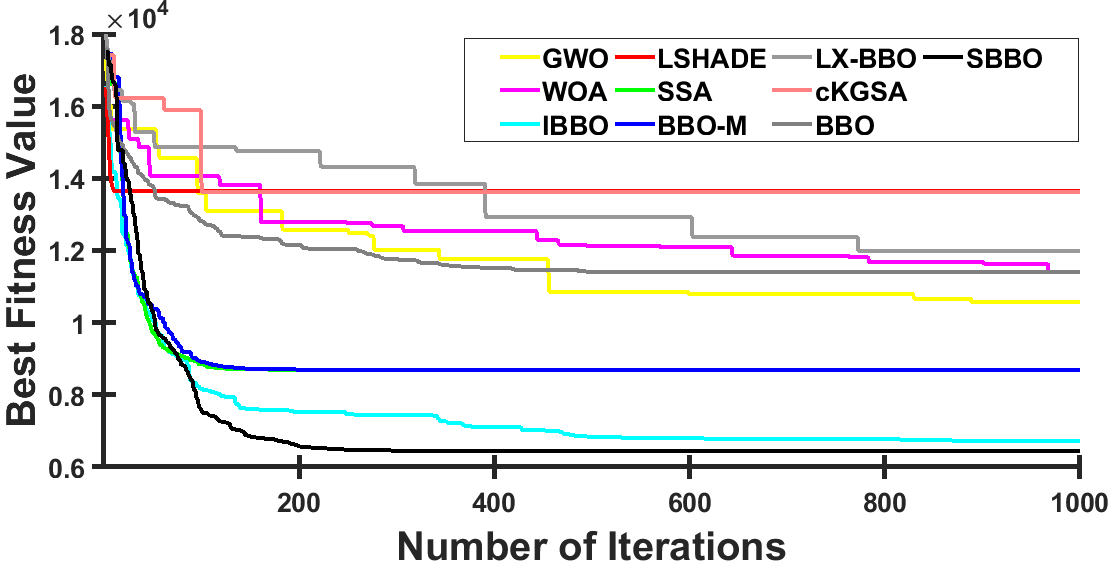
\includegraphics[width=0.45\linewidth]{s5}} 
\subfigure[]{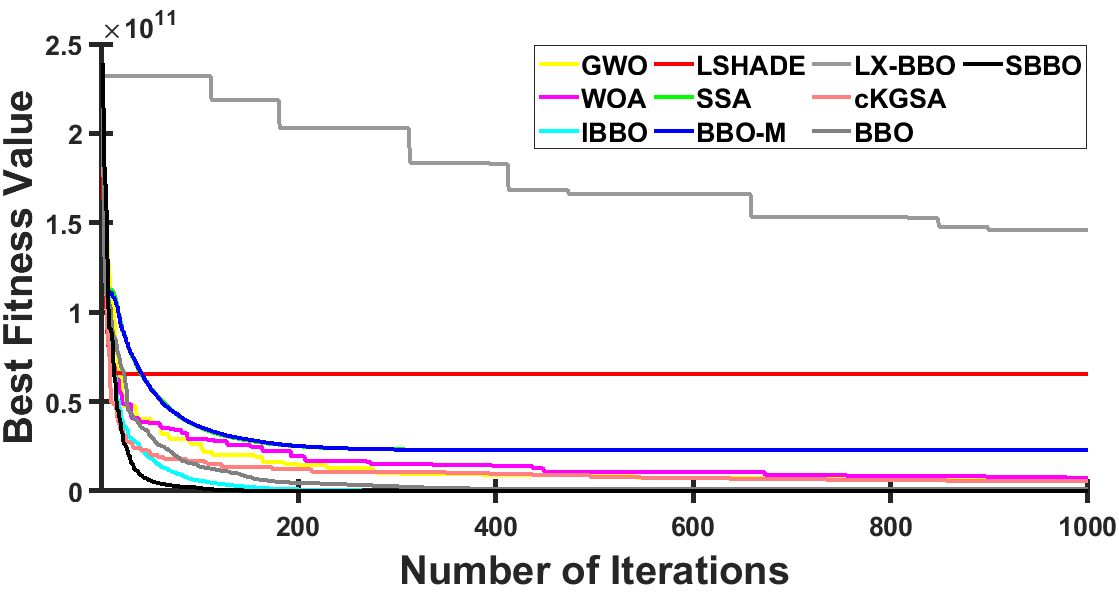
\includegraphics[width=0.45\linewidth]{s13}}
 \caption[Convergence trend of IBBO and SBBO with other considered Meta-heuristics standard benchmark problems]{\fontsize{10pt}{12pt}\selectfont Convergence trend of SBBO with other considered Meta-heuristics on standard benchmark problems, (a) Rastrigin ($F_{13}$) and (b) New Schwefel ($F_5$)}
\label{fig:cg1}
\end{figure}
\begin{figure}[h]
    \centering
 \subfigure[]{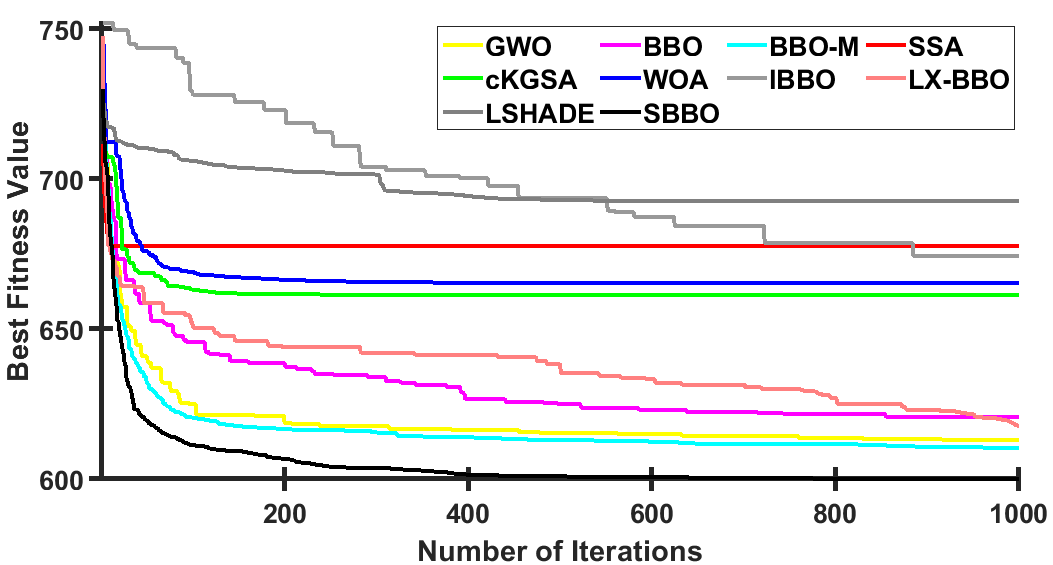
\includegraphics[width=0.45\linewidth]{6}}
\subfigure[]  {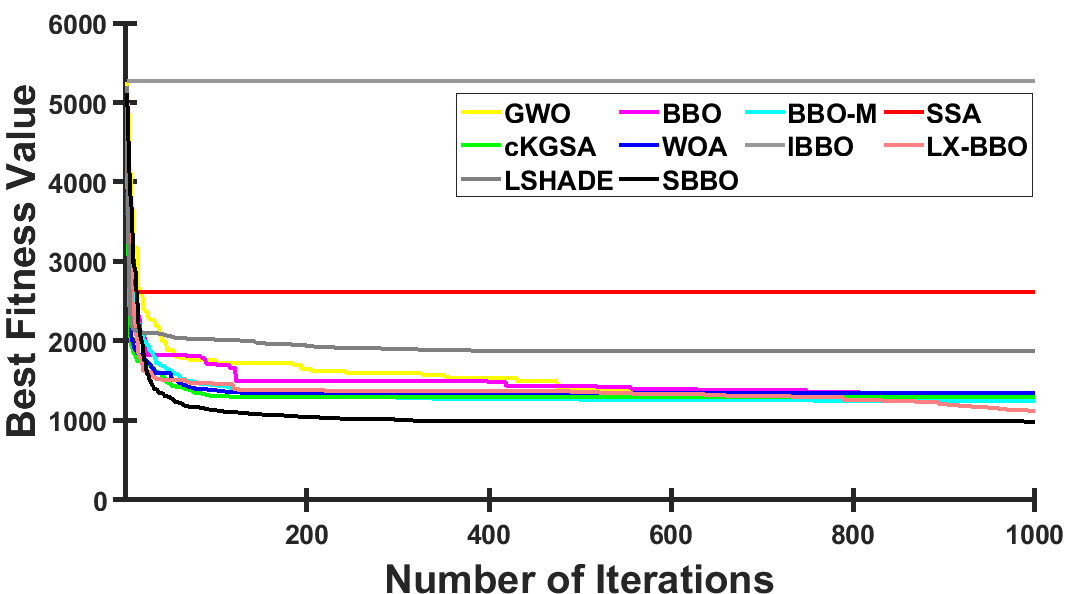
\includegraphics[width=0.45\linewidth]{7}}\\
\subfigure[]{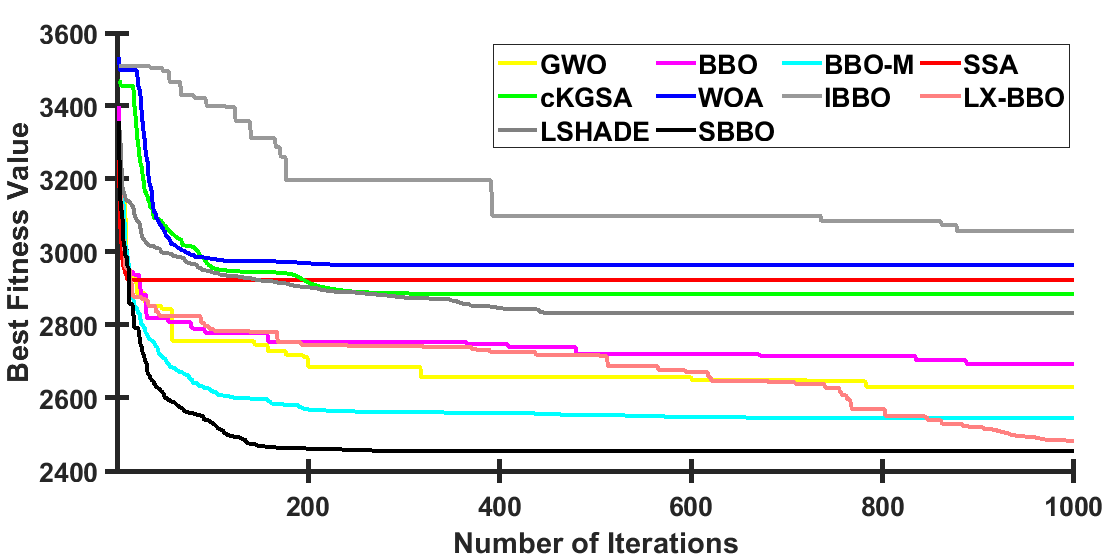
\includegraphics[width=0.45\linewidth]{21}}
\subfigure[]{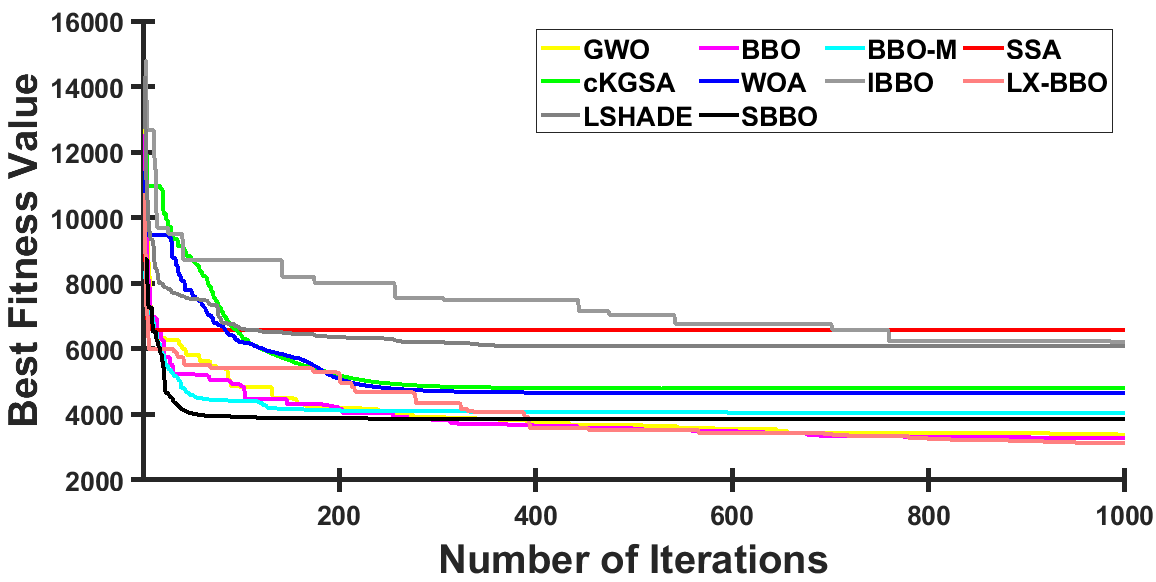
\includegraphics[width=0.45\linewidth]{16}}
 \caption[Convergence trend of  IBBO and SBBO with other considered Meta-heuristics on CEC 2017 benchmark problems]{\fontsize{10pt}{12pt}\selectfont Convergence trend of SBBO with other considered Meta-heuristics on CEC 2017 benchmark problems, (a) SR Expanded Scaffer's Function ($C_6$), (b) HF 6 (N=6)($C_{7}$), (c) CF 1 ($N=3$) ($C_{21}$), and (d) CF 5 ($N=5$) ($C_{25}$) }
\label{fig:cg2}
\end{figure}
The convergence behavior of an evolutionary algorithm is also a major component to be analyzed. Therefore, the convergence trends of the IBBO and SBBO have also been examined and compared with existing algorithms by plotting the convergence graph for standard benchmark problems and CEC 2017 benchmark problems.  Figure \ref{fig:cg1} \& \ref{fig:cg2} depict the convergence trends of all the algorithms for $200$, $400$, $600$, $800$, and $1000$ iterations on representative functions. The y-axes of all the convergence graphs shows the corresponding best fitness values and are represented in a logarithmic scales for standard bechmark problems and on linear scale for CEC 2017 benchmark problems. From the figures, it can be visualized that IBBO performs good for standard benchmark problems but it fails to show good behavior on CEC 2017 problems. However, SBBO has better convergence rate for almost all the unimodal, multi-modal, hybrid, and composite functions as compared to existing algorithms.  The exploration capability of SBBO is very good among all the other considered state-of-the-art methods as it converges gradually and finally optimum solution is achieved. Moreover, the convergence trend towards optimum is relatively more consistent. From all the presented results, it is elicited that the new SBBO is robust against local optimum and has attained a good balance between global and local search.


 
\subsection{Performance Analysis of SBBO based Histopathological Image Classification} \label{ch4:subsec:results2}
Since SBBO performs better than IBBO on various benchmark functions, it is used in the BOF to find the optimal visual words. The performance of SBBO based BOF method to classify histopathological images has been tested on two histopathological image datasets, namely the Blue histology dataset and ADL dataset as discussed in Section \ref{ch3:subsec:dataset}. Both the datasets are partitioned into two sets, namely training and validation sets using stratified random sampling. 

\subsubsection{Result Analysis on Blue Histology Dataset}
 The SBBO based BOF method is compared with two state-of-the-art methods, namely IB3 \cite{aha1991} and IKS2 \cite{lin2016} with original BOF \cite{caicedo2009} and BBO-M-BOF based classification methods. 
Further, IKS2 is used to find out the representative keypoints from the image set using iterative keypoint selection (IKS) method. The keypoints are eliminated if their distances from the representative keypoints are less than a predefined distance threshold. The distance threshold for IKS2 is taken as $0.57$. Moreover, the value of $K$ for IKS2 is $3$ as given in Lin et al.  \cite{lin2016}. 

Figure \ref{fig:cm_tissue} shows the confusion matrix for all the considered methods over blue histology dataset. In the figure, CT, ET, MT, and NT represent connective tissue, epithelium tissue, muscular tissue, and nervous tissue images respectively. The predicted class is given along the x-axis. The diagonal entries in the confusion matrices indicate the ratio of correct classification. The off-diagonal entries give the ratio of misclassification. From the figure, it can be visualized that the connective tissue images are correctly identified by BOF, IB3, IKS2, BBO-M-BOF, and SBBO-BOF based methods with an accuracy of $75\%$, $35\%$, $85\%$, $86\%$, and $69\%$ respectively. Although BOF, IKS2, and BBO-M-BOF  show better performance in the case of connective tissue images, they show degraded performance to classify the rest of the image categories. From the figure, it can be illustrated that the SBBO-BOF method identifies the rest of the image classes with the accuracy of $90\%$, $81\%$, and $49\%$ which are the best among other considered classification methods. This leads to an overall accuracy of SBBO-BOF based method to $72.23\%$ while BOF, IB3, IKS2, and BBO-M-BOF methods give only $47.5\%$, $40\%$, $50.63\%$, and $63.25\%$ accuracy. Therefore, based on the results, it can be stated the SBBO-BOF method outperforms. 

\begin{figure}
\centering
        \subfigure[BOF]{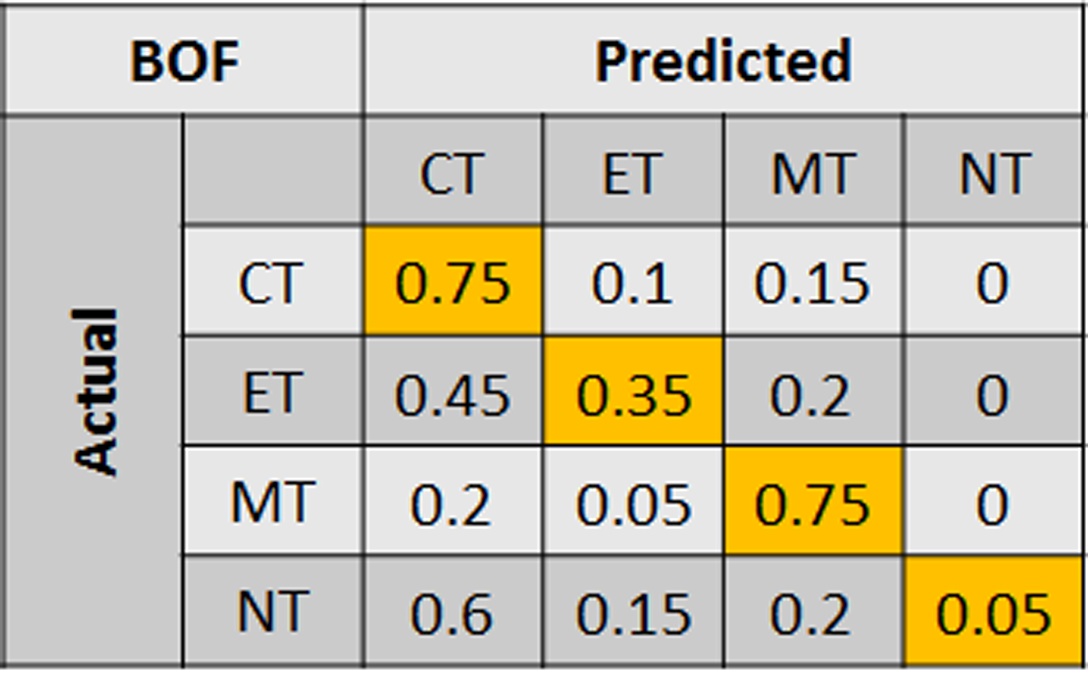
\includegraphics[width=0.31\linewidth]{CM_BOF}} \hspace{2mm}
            \subfigure[ IB3]{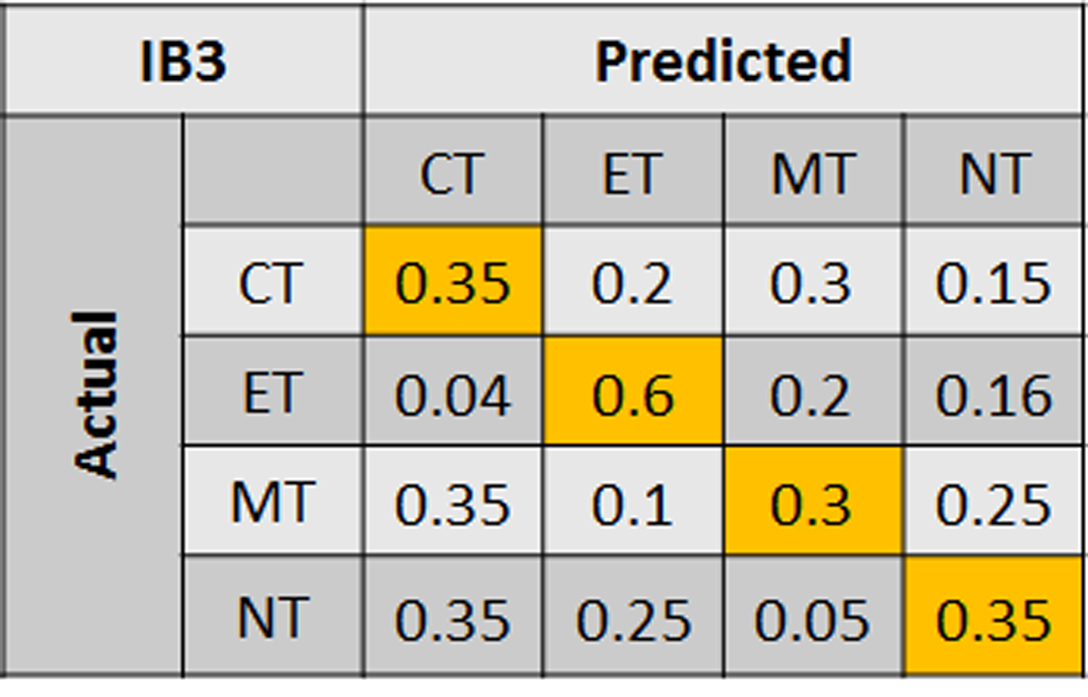
\includegraphics[width=0.31\linewidth]{CM_IB3}} \hspace{2mm}
        \subfigure[IKS2]{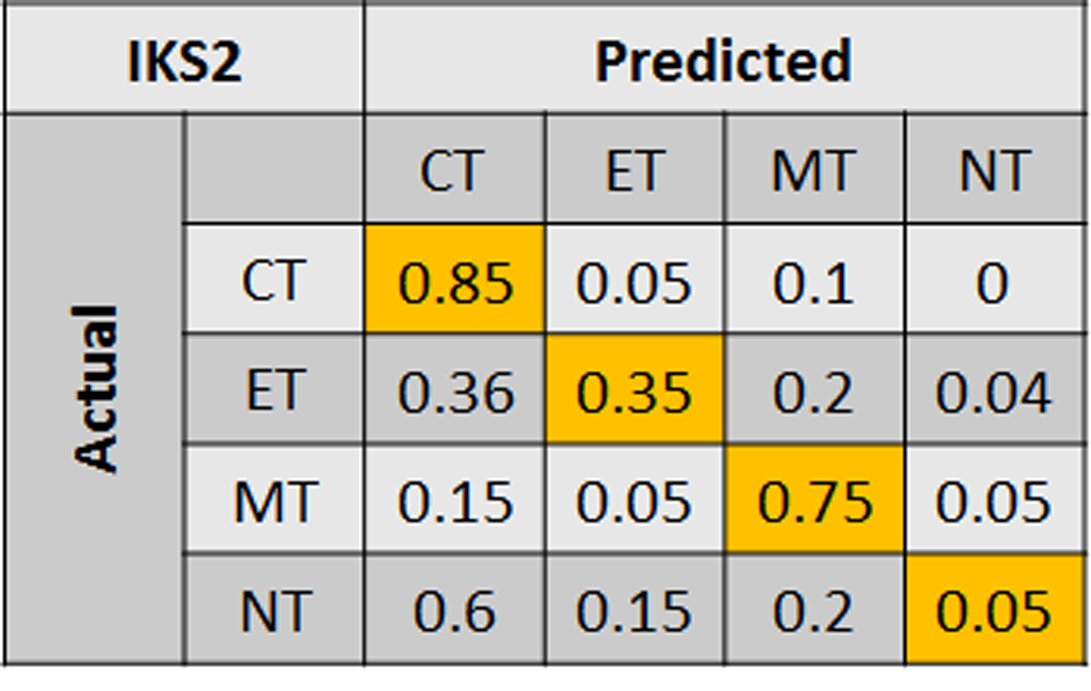
\includegraphics[width=0.31\linewidth]{CM_IKS2}} \\
        \subfigure[BBO-M-BOF]{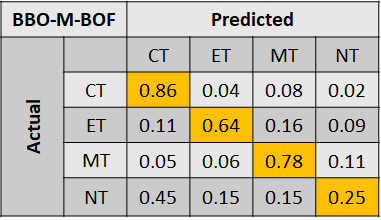
\includegraphics[width=0.31\linewidth]{CM_BBO-BOF}}\hspace{2mm}
        \subfigure[ SBBO-BOF]{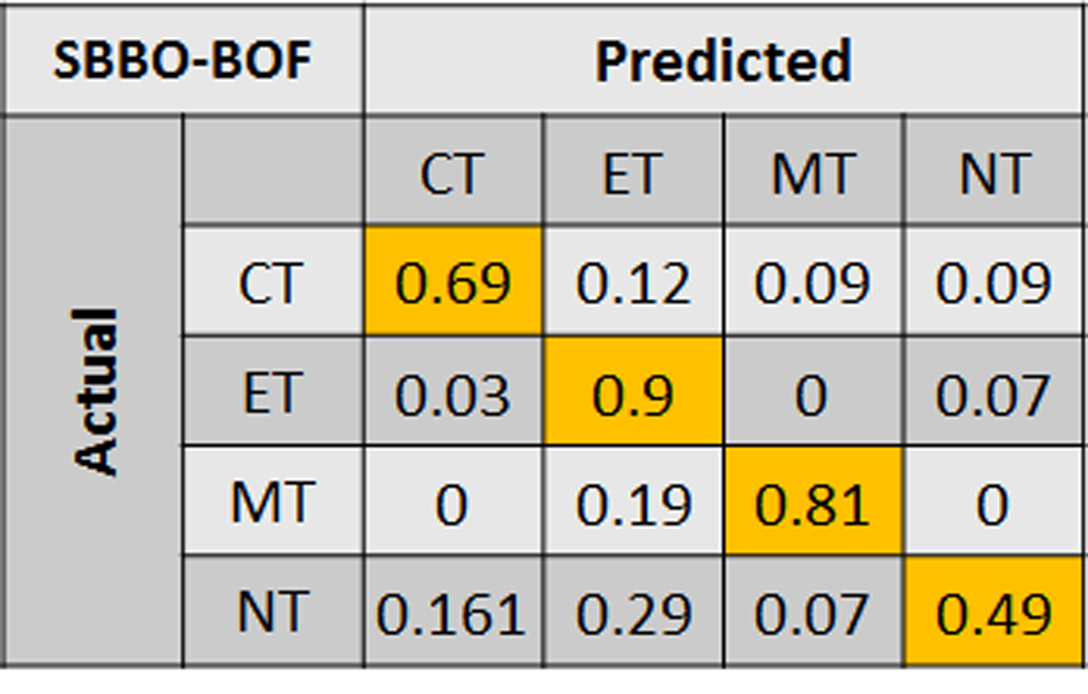
\includegraphics[width=0.31\linewidth]{CM_SBBO-BOF}}\hspace{2mm}
        
  \caption[The normalized confusion matrix for the blue histology tissue dataset for the five methods BOF, IB3, IKS2, BBO-M-BOF, and SBBO-BOF]{\fontsize{10pt}{12pt}\selectfont The normalized confusion matrix for the blue histology tissue dataset for the five methods BOF, IB3, IKS2, BBO-M-BOF, and SBBO-BOF.}
\label{fig:cm_tissue}
\end{figure}

Moreover, the comparative analysis of various performance matrices like recall, precision, F1-measure, and specificity are depicted in Table \ref{tab:perfor}.  The SBBO-BOF method shows better results for almost all the considered parameters. For muscle tissue class, it shows the best F1-measure equals to $0.82$ followed by connective, epithelial,  and nervous tissues respectively.  The overall accuracy of the new classification method increases by more than $10\%$ as compared to BBO-M-BOF based classification method which has the next highest accuracy. The results validate that the new SBBO-BOF classification method outperforms the other methods.

 \begin{table}[t]
\center
\scriptsize
    \caption[Comparative analysis of the SBBO-BOF based classification method]{\fontsize{10pt}{12pt}\selectfont Comparative analysis of the SBBO-BOF based classification method}
    \label{tab:perfor}
    {\renewcommand{\arraystretch}{1.2}
\begin{tabular}{|p{0.5in}|p{0.9in}|p{0.55in}|p{0.55in}|p{0.55in}|p{0.65in}|p{0.6in}|}
    \hline
  Category    &    Parameters    &    BOF    &    IB3    &    IKS2    &    BBO-M-BOF    &    SBBO-BOF    \\
 \hline

Muscle     &    Recall    &    0.750    &    0.300    &    0.750    &    0.750    &\textbf{    0.810    }\\
Tissue    &    Precision    &    0.577    &    0.353    &    0.600    &    0.667    &\textbf{    0.835    }\\
    &    F-measure    &    0.652    &    0.324    &    0.667    &    0.719    &\textbf{    0.822    }\\
    &    Specificity    &    0.817    &    0.817    &    0.831    &    0.870    &\textbf{    0.947    }\\
\hline
Connective     &    Recall    &    0.750    &    0.350    &    0.850    &\textbf{    0.850    }&    0.697    \\
Tissue    &    Precision    &    0.375    &    0.321    &    0.434    &    0.585    &\textbf{    0.783    }\\
    &    F-measure    &    0.500    &    0.335    &    0.574    &    0.696    &\textbf{    0.738    }\\
    &    Specificity    &    0.583    &    0.753    &    0.624    &    0.797    &\textbf{    0.937    }\\
\hline
Epithelial     &    Recall    &    0.350    &    0.600    &    0.368    &    0.684    &\textbf{    0.900    }\\
Tissue    &    Precision    &    0.538    &    0.522    &    0.583    &\textbf{    0.719    }&    0.600    \\
    &    F-measure    &    0.424    &    0.558    &    0.452    &    0.677    &\textbf{    0.720    }\\
    &    Specificity    &    0.900    &    0.817    &\textbf{    0.917    }&    0.917    &    0.800    \\
\hline
Nervous     &    Recall    &    0.050    &    0.350    &    0.050    &    0.200    &\textbf{    0.485    }\\
Tissue    &    Precision    &\textbf{    1.000    }&    0.385    &    0.357    &    0.532    &    0.754    \\
    &    F-measure    &    0.095    &    0.366    &    0.088    &    0.340    &\textbf{    0.590    }\\
    &    Specificity    &    1.000    &    0.813    &\textbf{    0.969    }&    0.927    &    0.946    \\
    &    Overall Accuracy    &    47.5    &    40    &    50.63    &    63.25    &\textbf{    72.23    }\\

\hline
 \end{tabular}}
\end{table}

\begin{figure}[h]
\centering
\subfigure[Connective Tissue]{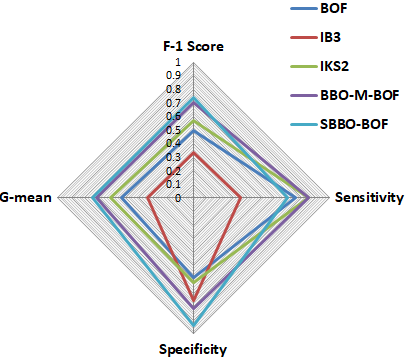
\includegraphics[width=0.3\linewidth]{CT_radar}}
\subfigure[ Epithelial Tissue]{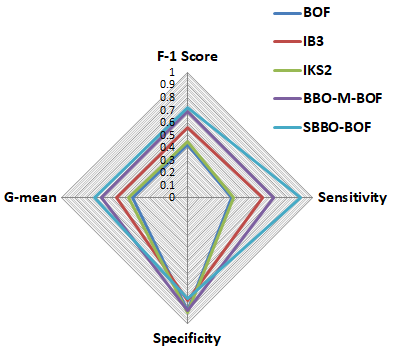
\includegraphics[width=0.3\linewidth]{ET_radar}}
\subfigure[Muscle Tissue]{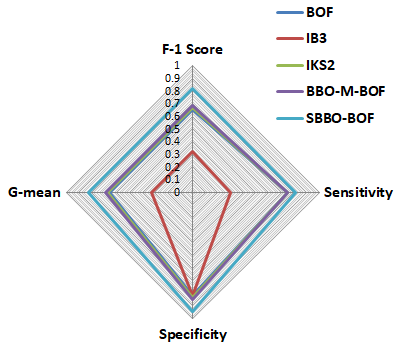
\includegraphics[width=0.3\linewidth]{MT_radar}} 
\subfigure[Nervous Tissue]{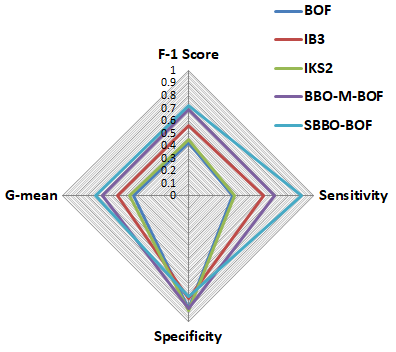
\includegraphics[width=0.3\linewidth]{NT_radar}} 
 \caption[ Radar chart for average results obtained by SVM classifier on Blue histology dataset by considering F1 score, G-mean, sensitivity, and specificity]{\fontsize{10pt}{12pt}\selectfont Radar chart for average results obtained by SVM classifier on Blue histology dataset. }
\label{ch4:fig:T3tissue}
\end{figure}


Furthermore, a comparison of the F1 score, G-mean, sensitivity, and specificity is represented using the radar chart as shown in Figure \ref{ch4:fig:T3tissue}. The radar chart shows that the method with the largest area and symmetrical shape performs better than others. From the figure, it is visualized that for muscle tissue, the area covered by the SBBO-BOF method is larger than other methods on all four considered aspects while for other tissue classes, the covered area is larger as compared with the other methods. These results validate the effectiveness of the SBBO-BOF method in the image classification problem for the Blue histology dataset.


\subsubsection{Result Analysis on ADL dataset}
 
The classification efficiency of the new method has been observed for all the three different types of organ images i.e., Kidney, Lung, and Spleen in the ADL dataset. The results of the SBBO-BOF method have been compared with three state-of-the-art methods, namely SVM \cite{Chapelle1999}, SRC \cite{wright2009}, and SHIRC which are already analyzed in the literature on ADL dataset by Srinivas et al. \cite{srinivas2014}. SVM is used for decision making in the classification process. For feature extraction, the state-of-the-art method, namely WND-CHARM \cite{orlov2008} is used. Further, SRC is the classification method with a single channel sparse representation of RGB images. Moreover, SHIRC is the extension of the SRC approach and is known as a simultaneous sparsity model for multi-channel histopathological images which designs three color dictionaries for RGB channels. 

\begin{table}
\renewcommand{\arraystretch}{1.2}
\scriptsize
\begin{minipage}[b]{0.5\textwidth}
    \caption[The confusion matrix for kidney image classification obtained by the SBBO-BOF method]{\fontsize{10pt}{12pt}\selectfont The confusion matrix for kidney image classification obtained by the SBBO-BOF method}
    \label{tab:cm_kid}
\renewcommand{\arraystretch}{1.2}
\begin{tabular}{|p{0.7in}|p{0.45in}|p{0.6in}|p{0.7in}|}
\hline
Class    &    Healthy    &    Inflammatory    &    Method    \\
\hline
Healthy    &    0.6925    &    0.3075    &    SVM    \\
    &    0.875    &    0.125    &    SRC    \\
    &    0.825    &    0.175    &    SHIRC    \\
    &    \textbf{0.89}    &    0.11    &    SBBO-BOF    \\
\hline
Inflammatory    &    0.2812    &    0.7188    &    SVM    \\
    &    0.25    &    0.75    &    SRC    \\
    &    0.1667    &    0.8333    &    SHIRC    \\
    &    0.175    &    \textbf{0.875}    &    SBBO-BOF    \\
\hline
 \end{tabular}
  \end{minipage}\qquad
 \begin{minipage}[b]{0.50\textwidth}
 \scriptsize
    \caption[ The confusion matrix for lung image classification obtained by the SBBO-BOF method]{\fontsize{10pt}{12pt}\selectfont The confusion matrix for lung image classification obtained by the SBBO-BOF method}
    \label{tab:cm_lg}
{\renewcommand{\arraystretch}{1.2}    
\begin{tabular}{|p{0.7in}|p{0.45in}|p{0.6in}|p{0.7in}|}
    \hline
Class    &    Healthy    &    Inflammatory    &    Method    \\
\hline
Healthy    &    0.8875    &    0.1125    &    SVM    \\
    &    0.725    &    0.275    &    SRC    \\
    &    0.75    &    0.25    &    SHIRC    \\
    &\textbf{    0.92    }&    0.08    &    SBBO-BOF    \\
\hline
Inflammatory    &    0.372    &    0.6238    &    SVM    \\
    &    0.2417    &    0.7853    &    SRC    \\
    &    0.15    &    0.85    &    SHIRC    \\
    &    0.15    &\textbf{    0.85    }&    SBBO-BOF    \\
\hline
 \end{tabular}}
\end{minipage} 
\end{table}


 \begin{table}
\scriptsize
\centering
 \caption[The confusion matrix for spleen image classification obtained by the SBBO-BOF method]{\fontsize{10pt}{12pt}\selectfont The confusion matrix for spleen image classification obtained by the SBBO-BOF method}
    \label{tab:cm_spl}
{\renewcommand{\arraystretch}{1.2}    
\begin{tabular}{|p{0.7in}|p{0.45in}|p{0.6in}|p{0.7in}|}
    \hline
Class    &    Healthy    &    Inflammatory    &    Method    \\
\hline
Healthy    &    0.5112    &    0.488    &    SVM    \\
    &    0.7083    &    0.2917    &    SRC    \\
    &    0.65    &    0.35    &    SHIRC    \\
    &\textbf{    0.828    }&    0.172    &    SBBO-BOF    \\
\hline
Inflammatory    &    0.1275    &    0.8725    &    SVM    \\
    &    0.2083    &    0.7917    &    SRC    \\
    &    0.1167    &    0.8833    &    SHIRC    \\
    &    0.1    &\textbf{    0.9    }&    SBBO-BOF    \\
\hline
 \end{tabular}}
\end{table}
\begin{figure}
\centering
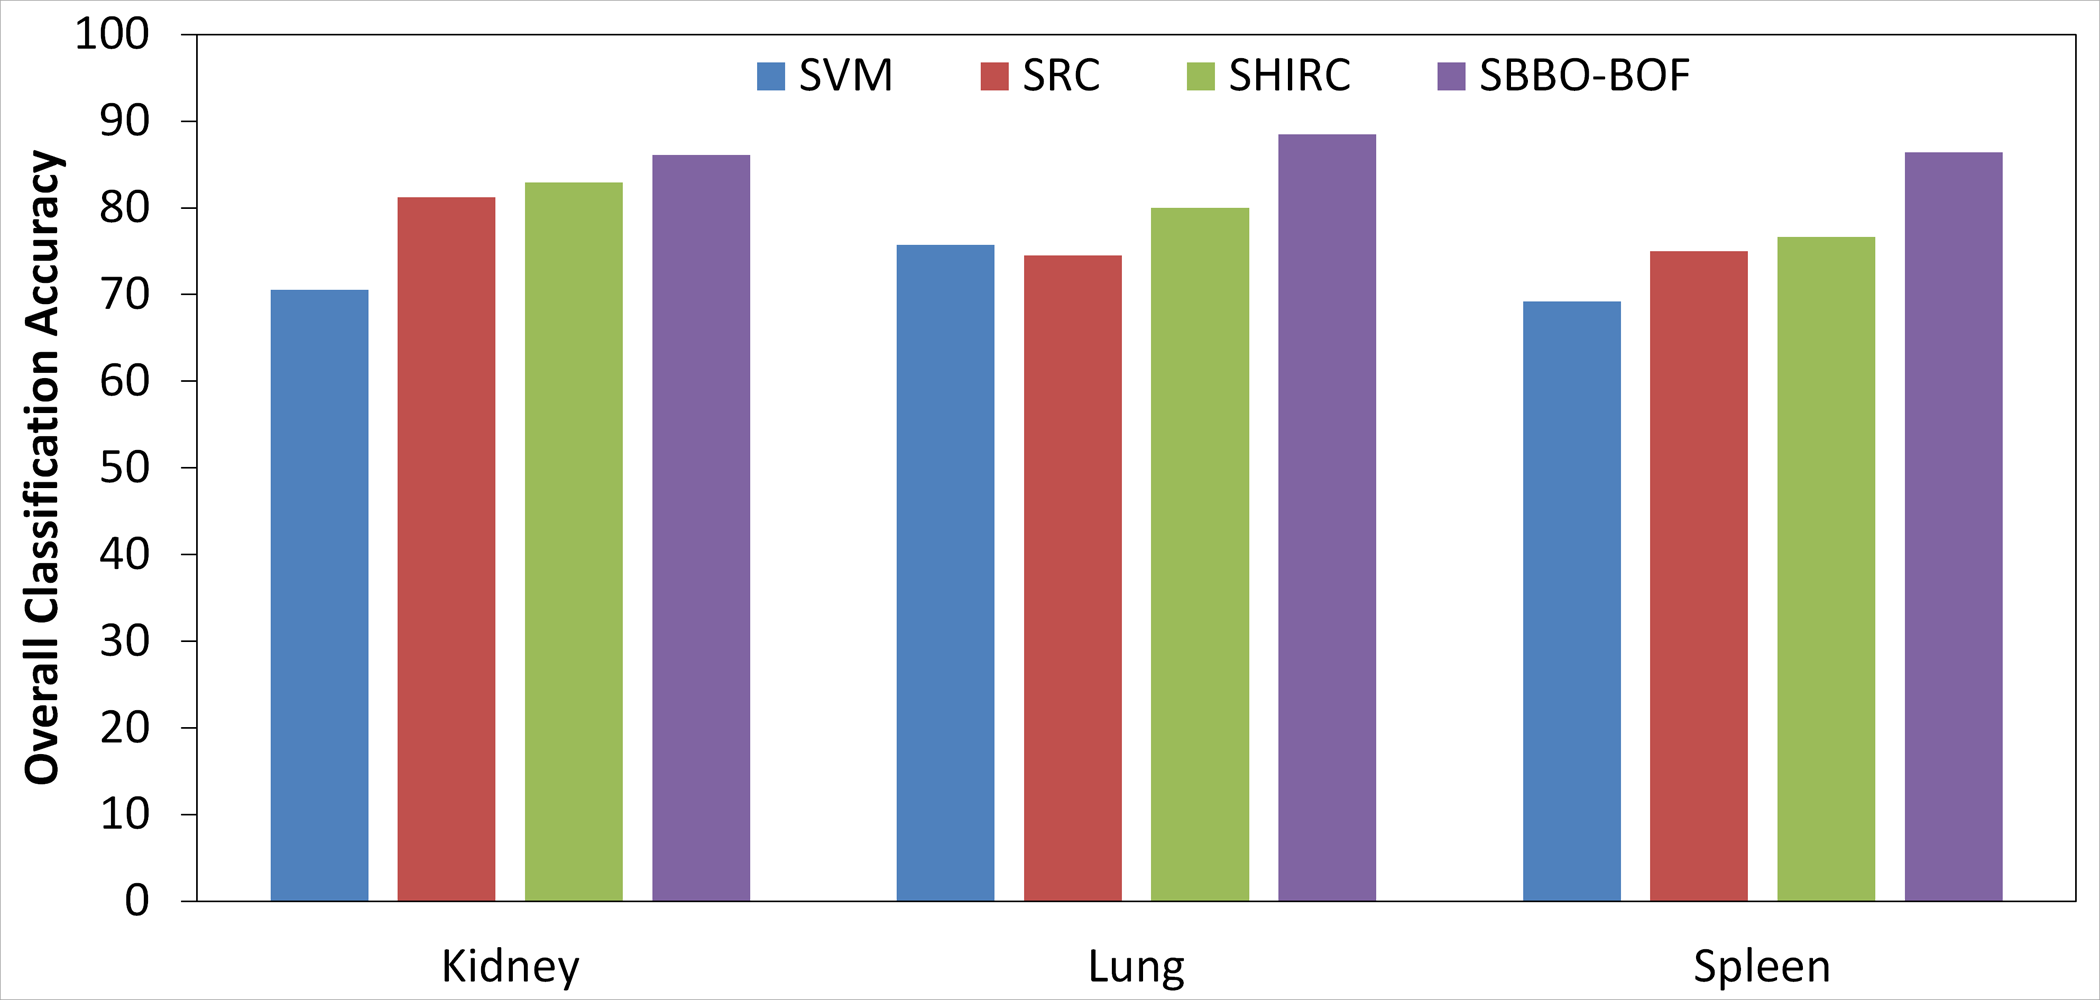
\includegraphics[width=0.7\textwidth]{adlbar}
\caption[The overall classification accuracy of the considered methods for ADL dataset in form of bar chart]{\fontsize{10pt}{12pt}\selectfont The overall classification accuracy of the considered methods for ADL dataset in form of bar chart}
\label{fig:adlbar}
\end{figure}

Tables \ref{tab:cm_kid} to \ref{tab:cm_spl} show the confusion matrices for all the considered methods over three datasets as mentioned above. From the tables, it can be observed that the SBBO-BOF method identifies the healthy kidney, lung, and spleen images with an accuracy of $89\%$, $92\%$, and $82.8\%$ respectively. Likewise, the accuracy of $87.5\%$, $85\%$, and $90\%$ is observed for inflamed kidney, lung, and spleen images. All the accuracy is better than considered methods. Moreover, the overall average accuracy of the SBBO-BOF method is $87\%$ followed by SHIRC method with an average accuracy of $79.86\%$. The average accuracy of all other considered methods is depicted in Figure \ref{fig:adlbar}. Furthermore, a comparison of the F1 score, G-mean, sensitivity, and specificity is also represented using radar charts as shown in Figure \ref{ch4:fig:T3adl}. These figures also show the effectiveness of the SBBO-BOF method over other methods. 

\begin{figure}[t!]
\centering
\subfigure[Spleen]{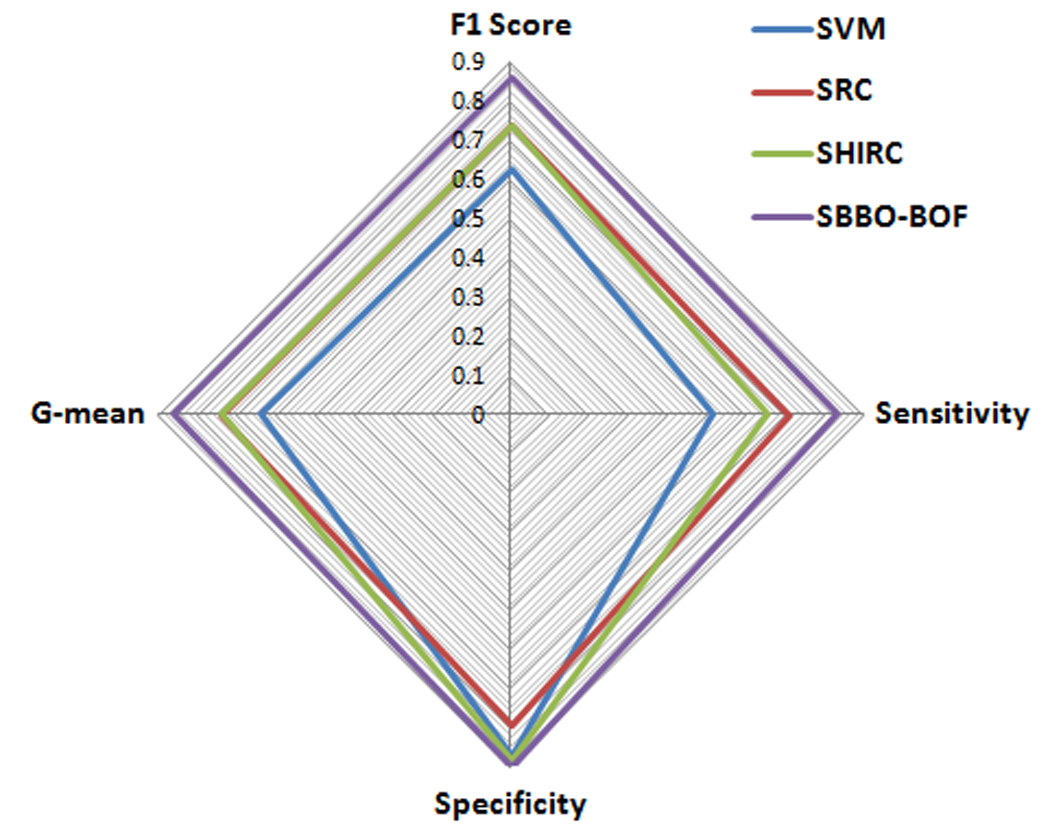
\includegraphics[width=0.3\linewidth]{Spleen_radar}}
\subfigure[ Kidney]{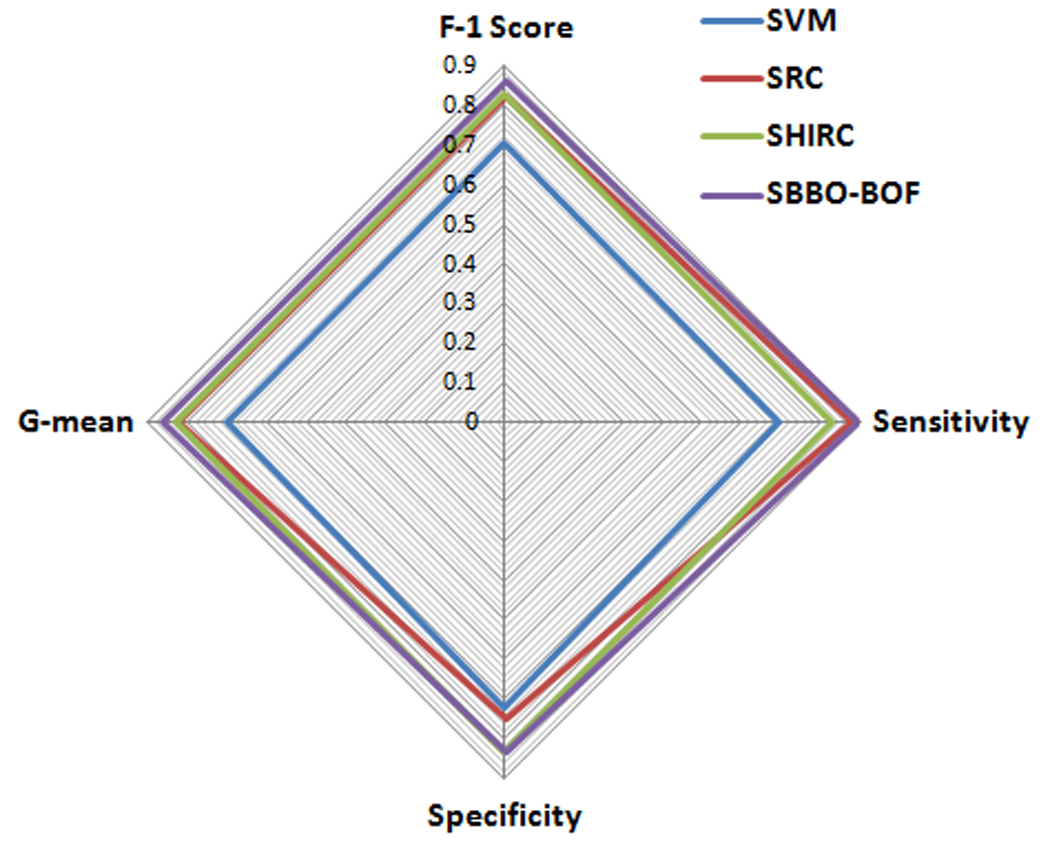
\includegraphics[width=0.3\linewidth]{Kidney_radar}}
\subfigure[Lung]{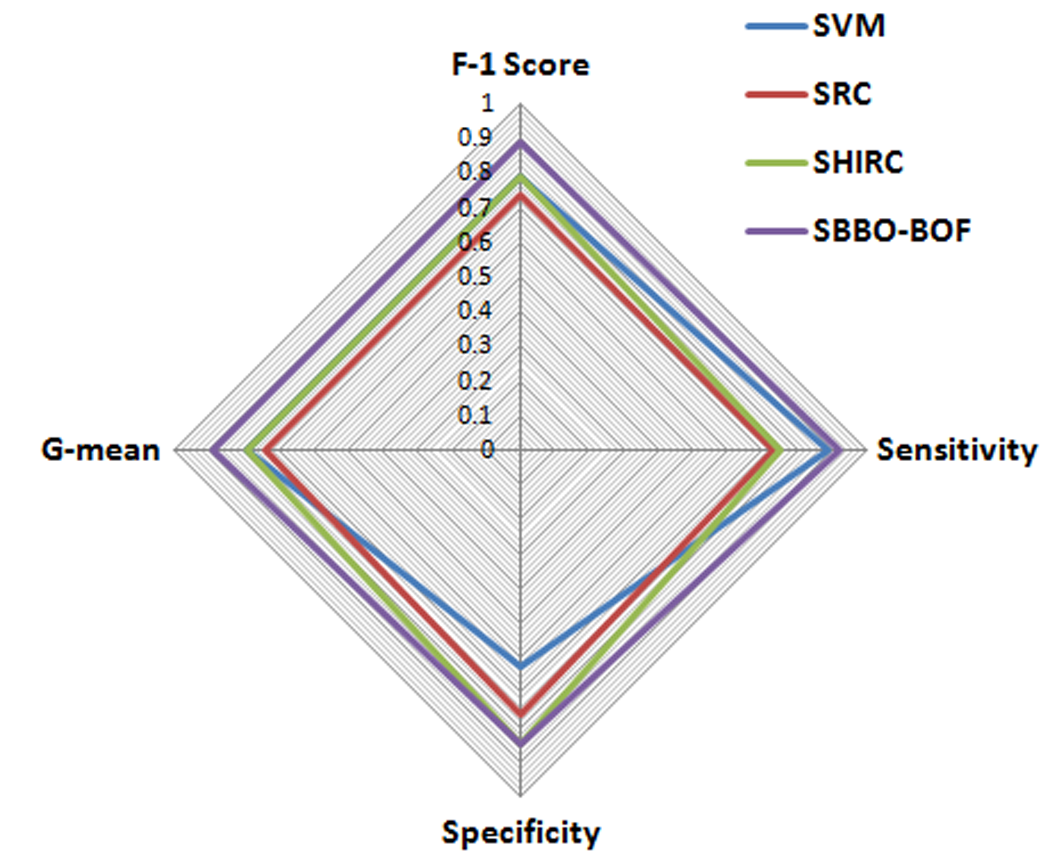
\includegraphics[width=0.3\linewidth]{l_radar}} 
 \caption[Radar chart for average results on Spleen dataset, Kidney dataset, and Lung dataset]{\fontsize{10pt}{12pt}\selectfont Radar chart for average results on (a) Spleen dataset, (b) Kidney dataset, and (c) Lung dataset}
\label{ch4:fig:T3adl}
\end{figure}

\subsubsection{Computational Complexity of SBBO based BOF Method}
The computational cost of the SBBO-BOF method has also been measured asymptotically and described below:
\begin{itemize}
\item   The computational cost of K-means is $O(N^2)$ \cite{pakhira2004}, where $N$ refers to the descriptor count.

\item For the calculation of fitness value, the sum of squared Euclidean distances between the cluster centers and the corresponding descriptors are considered. Hence, the computational cost of the fitness calculation becomes $O (N \times C)$, where $C$ represents the cluster count.

\item  Since, the SBBO only enhances the mutation operator of BBO, therefore its computational cost will be similar to BBO which is $O(P^2)$ \cite{wang2014}, where $P$ represents the size of the population.

\end{itemize}

Therefore, the overall computational complexity of the new SBBO-BOF method can be given as $O(N^2 +N \times C+P^2)$. As the descriptor count ($N$) for the histopathological images is much larger than the population size ($P$), therefore, the worst case time complexity of the SBBO-BOF method is $O(N^2)$.


 \section{Summary}\label{sec:5}
This chapter presents two new variants of BBO, namely IBBO and SBBO and analyze their performance on standard and CEC 2017 benchmark problems. IBBO performs well for standard benchmark problems but it fails to optimize the CEC 2017 benchmark problems. However, SBBO outperforms the other considered algorithms on both types of benchmark problems. Therefore, SBBO is further applied to find the optimal visual words in the BOF method and the modified SBBO based BOF method (SBBO-BOF) has been tested and validated on two histopathological image datasets for the classification of tissue images. The SBBO-BOF method outperforms other image classification methods in terms of average accuracy, recall, precision, and F1-measure. The results depict that the SBBO-BOF method attains a high average accuracy of $72.23\%$ and $87\%$ for blue histology dataset and ADL dataset respectively. However, the SBBO-BOF codebook construction method is computationally expensive. Therefore, in the next chapter,  a computationally efficient grey relational analysis based codebook construction method is introduced.







